%!TEX root = main.tex

\section{Appendix}

\subsection{Construction of {\PSST} from {\regexp}}

\paragraph{Case $e =\emptyset$ (see Figure~\ref{fig-reg2pfa-0})} $\cT_\emptyset = (\{q_{\emptyset, 0}\}, \Sigma, \{x_{\emptyset}\}, \delta_\emptyset, \tau_\emptyset, E_\emptyset, q_{\emptyset, 0}, (\emptyset, \emptyset))$, where there are no transitions out of $q_{\emptyset,0}$, namely, $\delta_\emptyset(q_{\emptyset, 0}, a) = ()$ for every $a \in \Sigma$, $\tau_\emptyset(q_{\emptyset, 0}) = ((); ())$, and $E_\emptyset$ is vacuous here.
%$\delta_\emptyset(q_{\emptyset, 0}, a) = ()$ for every $a \in \Sigma$, $\tau_\emptyset(q_{\emptyset, 0}) = ((); ())$, and $E_\emptyset$ is vacuous here. 


\paragraph{Case $e = \varepsilon$ (see Figure~\ref{fig-reg2pfa-0})} $\cT_\varepsilon = (\{q_{\varepsilon, 0}, f_{\varepsilon,0}\}, \Sigma, \{x_\varepsilon\}, \delta_\varepsilon, \tau_\varepsilon, E_\varepsilon, q_{\varepsilon,0}, (\{f_{\varepsilon,0}\}, \emptyset))$, 
%
where 
%$\delta_\varepsilon(q_{\varepsilon,0}, a) = \delta_\varepsilon(f_{\varepsilon,0}, a) = ()$ for every $a \in \Sigma$, 
$\tau_\varepsilon(q_{\varepsilon,0}) = ((f_{\varepsilon,0}); ())$, %for each transition $(q, a, q')$, 
and $E_\varepsilon(q_{\varepsilon,0}, \varepsilon, f_{\varepsilon,0})(x) = \varepsilon$. Note $F_2 = \emptyset$ here. 

\paragraph{Case $e = a$ (see Figure~\ref{fig-reg2pfa-0})} $\cT_a = (\{q_{a,0}, q_{a,1}, f_{a,0}\}, \Sigma, \{x_a\}, \delta_a, \tau_a, E_a, q_{a,0}, (\emptyset, \{f_{a,0}\}))$, where 
%$\delta_a(q_{a,0}, b) = ()$ for every $b \in \Sigma$, 
$\tau_a(q_{a,0}) = ((q_{a,1}); ())$, 
%
$\delta_a(q_{a,1}, a) = (f_{a,0})$, 
%$\delta_a(q_{a,1}, b) = ()$ for every $b \in \Sigma \setminus \{a\}$,
%
%$\tau_a(q_{a,1}) = ((); ())$, and $\tau_a(f_{a,0}) = ((); ())$, 
%
$E_a(q_{a,0}, \varepsilon, q_{a,1})(x_a) = \varepsilon$, and $E_a(q_{a,1}, a, f_{a,0})(x_a) =x_aa$. Note $F_1 = \emptyset$ here. 
%		
\begin{figure}[ht]
	\centering
	%\rule{\linewidth}{0cm}
	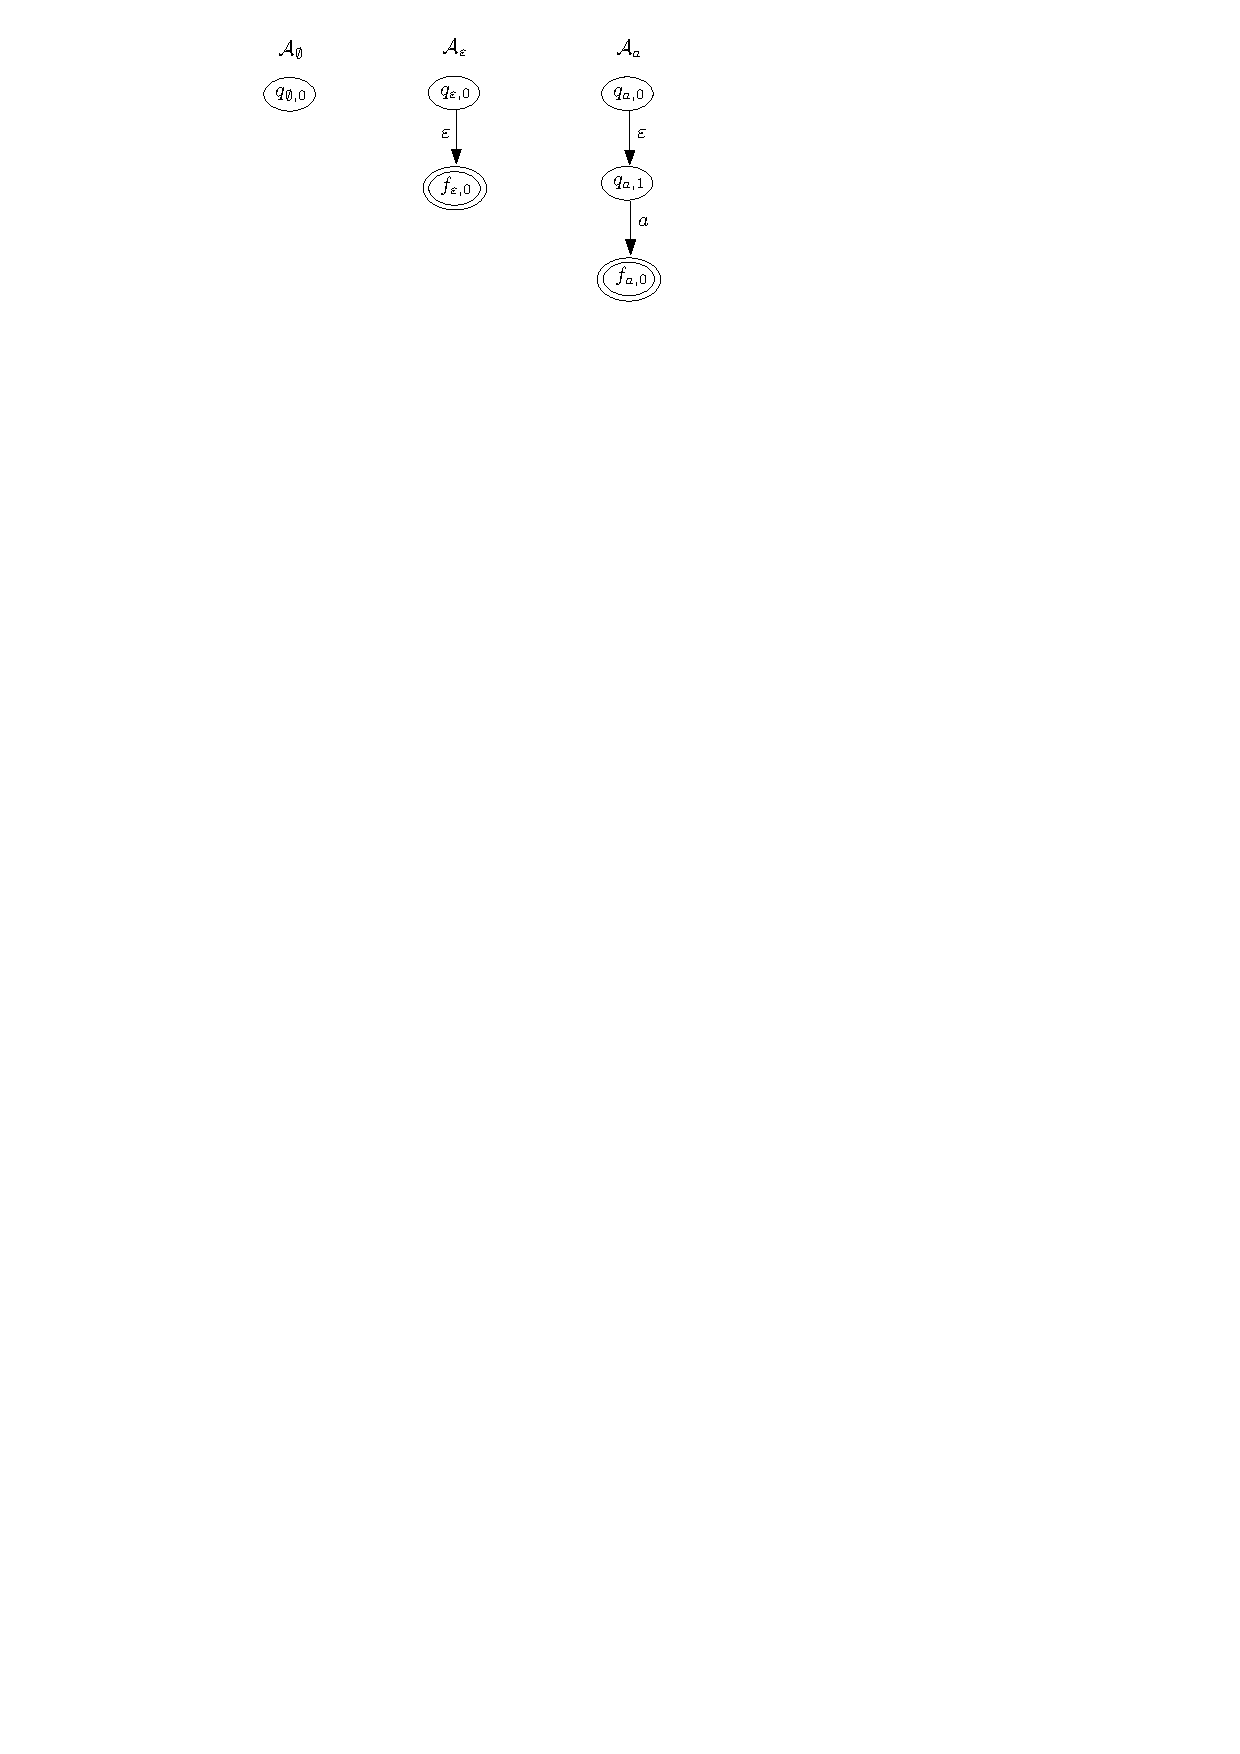
\includegraphics[width = 0.4\textwidth]{reg2pfa-0.pdf}
	\caption{The PSST $\cT_{\emptyset}$, $\cT_{\varepsilon}$, and $\cT_{a}$ }
	\label{fig-reg2pfa-0}
\end{figure}

\paragraph{Case $e = [e_1 \concat e_2]$} 
For $i \in \{1,2\}$, let  
$\cT_{e_i} = (Q_{e_i}, \Sigma, X_{e_i}, \delta_{e_i}, \tau_{e_i}, E_{e_i}, q_{e_i,0}, (F_{e_i,1}, F_{e_i,2}))$. Moreover, let us assume that $X_{e_1}\cap X_{e_2}=\emptyset$.
Then $\cT_e$ is obtained from $\cT_{e_1} \concat \cT_{e_2}$ (the concatenation of $\cT_{e_1}$ and $\cT_{e_2}$, see Figure~\ref{fig-psstconcat}) by adding a string variable $x_e$, a fresh state $q_{e,0}$ as the initial state, the transition $\tau_e(q_{e,0}) = (q_{e_1,0})$, and the assignments $E_e(q_{e,0}, \varepsilon, q_{e_1,0})(x_e) = \varepsilon$, $E_e(p, a, q)(x_e) = x_e a$ for every transition $(p, a, q)$ in $\cT_{e_1}$, $\cT_{e_2}$, and $\cT'_{e_2}$ (where $a \in \Sigma^\varepsilon$).
%%%%%%%%%%%%%%%%%%%%%%%%%%%%%%
\OMIT{
	Suppose that
	$\cT'_{e_2} = (Q'_{e_2}, \Sigma, X_{e_2}, \delta'_{e_2}, \tau'_{e_2}, E_{e_2}', q'_{e_2,0}, (F'_{e_2, 1}, F'_{e_2,2}))$ is a fresh copy of $\cT_{e_2}$, but with the string variables of $\cT_{e_2}$ kept unchanged. 
	Then 
	%
	\[\cT_e = ( Q_{e_1} \cup Q_{e_2} \cup Q'_{e_2} \cup \{q_{e,0}\}, \Sigma, X_e, \delta_e, \tau_e, q_{e_1,0}, (F_{e_2,1}, F_{e_2,2} \cup F'_{e_2,1} \cup F'_{e_2,2}))\] where 
	\begin{itemize}
		\item $X_e = X_{e_1} \cup X_{e_2} \cup \{x_e\}$,
		%
		\item $\delta_e$ is defined as follows:
		\begin{itemize}
			\item for every $a \in \Sigma$, $\delta_e(q_{e,0}, a) = ()$,
			%
			\item for every $i \in \{1,2\}$, $q \in Q_{e_i}$ and $a \in \Sigma$, $\delta_e(q, a) = \delta_{e_i}(q, a)$,
			%
			\item for every $q' \in Q'_{e_2}$ and $a \in \Sigma$, $\delta_e(q', a) = \delta'_{e_2}(q',a)$, 
		\end{itemize}
		%
		\item $\tau_e$ is defined as follows: 
		\begin{itemize}
			\item $\tau_e(q_{e,0}) = ((q_{e_1,0}); ())$;
			%    
			\item for every $q \in Q_{e_2}$, $\tau_e(q) = \tau_{e_2}(q)$ and $\tau_e(q') = \tau'_{e_2}(q')$, 
			%
			\item for every $q \in Q_{e_1} \setminus (F_{e_1,1} \cup F_{e_1,2})$, $\tau_e(q) = \tau_{e_1}(q)$, 
			\item for every $f_{e_1,1} \in F_{e_1,1}$, $\tau_e(f_{e_1,1}) = ((q_{e_2,0}); ())$, 
			\item for every $f_{e_1,2} \in F_{e_1,2}$, $\tau_e(f_{e_1,2}) = ((q'_{e_2,0}), ())$,
		\end{itemize}
		%
		\item $E_e$ is defined as follows: 
		\begin{itemize}
			\item $E_e(q_{e,0}, \varepsilon, q_{e_1,0})(x_e) = \varepsilon$, and for every $x \in X_{e_1} \cup X_{e_2}$, $E_e(q_{e,0}, \varepsilon, q_{e_1,0})(x) = x$,
			%
			\item for each $i\in \{1,2\}$, transition $(p, a, q)$ in $\cT_{e_i}$ (where $a \in \Sigma^\varepsilon$), $E_e(p, a, q)(x_e) = x_e a$, moreover, for every $x\in X_{e_i}$, $E_e(p, a, q)(x) = E_{e_i}(p, a, q)(x)$,
			%
			\item for each transition $(p', a, q')$ in $\cT'_{e_2}$, $E_e(p', a, q')(x_e) = x_e a$, and for every $x \in X_{e_2}$, $E_e(p', a, q')(x) = E_{e_2}(p, a, q)(x)$,
			\item for $f_{e_1,1} \in F_{e_1,1}$ and $f_{e_1,2} \in F_{e_1,2}$, $E_e(f_{e_1,1},\varepsilon,q_{e_2,0})(x_{e_2}) = E_e(f_{e_1,2},\varepsilon,q'_{e_2,0})(x_{e_2}) =\varepsilon$, and for every $x \in X_e \setminus \{x_{e_2}\}$, $E_e(f_{e_1,1},\varepsilon,q_{e_2,0})(x) = E_e(f_{e_1,2},\varepsilon,q'_{e_2,0})(x) = x$.
		\end{itemize}
	\end{itemize}
}
%%%%%%%%%%%%%%%%%%%%%%%%%%%%%%
% Fig.~\ref{fig-reg2pfa-2} depicts the construction. 
\begin{figure}[ht]
	\centering
	%\rule{\linewidth}{0cm}
	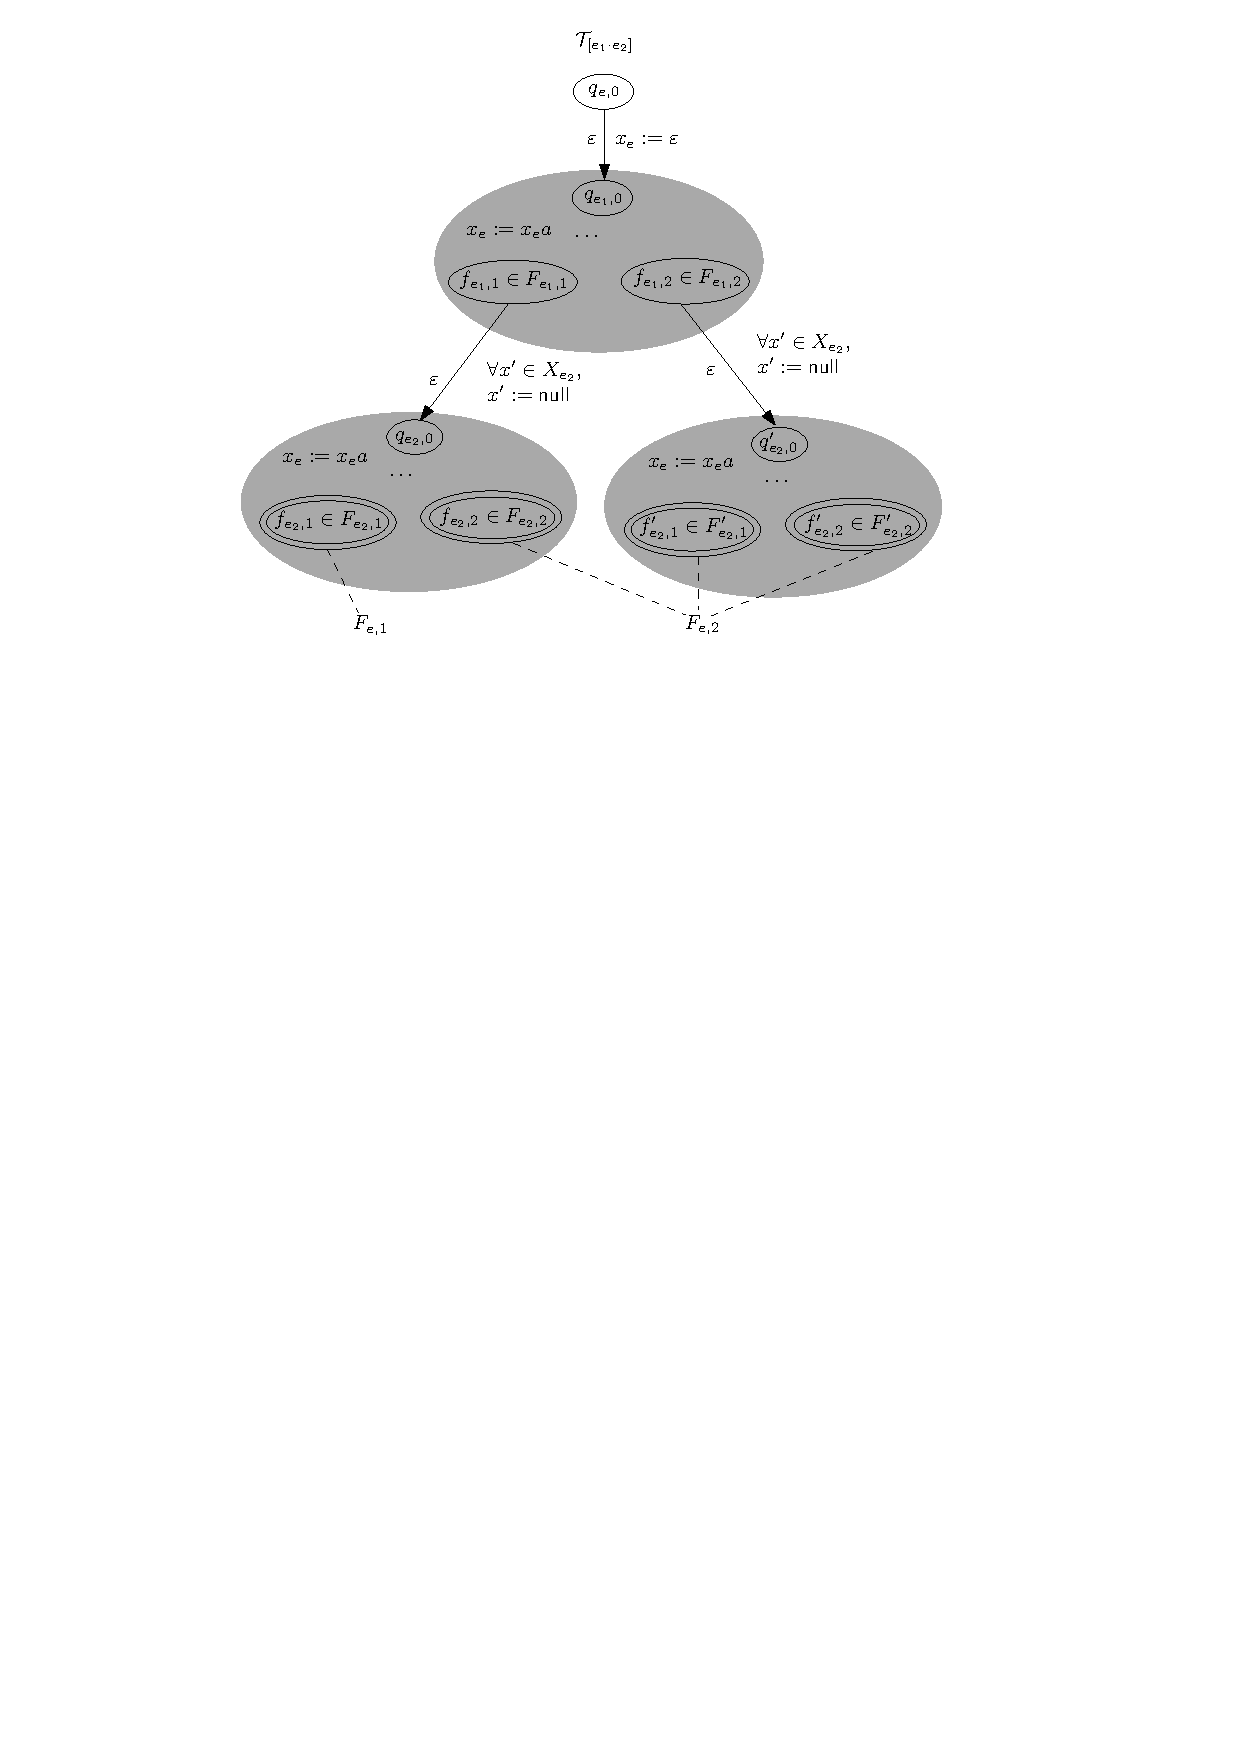
\includegraphics[width = 0.6\textwidth]{reg2pfa-2.pdf}
	\caption{The PSST $\cT_{[e_1\concat e_2]}$}
	\label{fig-reg2pfa-2}
\end{figure}  

\paragraph{Case $e = [e_1^{+}]$}  We first construct $\cT_{e_1}$ and $\cT^-_{[e^\ast_1]}$, where $\cT^-_{[e^\ast_1]}$ is obtained from $\cT_{[e^\ast_1]}$ by dropping the string variable $x_{[e^\ast_1]}$. Therefore, $\cT_{e_1}$ and $\cT^-_{[e^\ast_1]}$ have the same set of string variables, $X_{e_1}$. Then we construct $\cT_{e}$ by adding into $\cT_{e_1} \concat \cT^-_{[e^\ast_1]}$, the concatenation of $\cT_{e_1}$ and $\cT^-_{[e^\ast_1]}$, a fresh state $q_{e,0}$ as the initial state, and the transitions $\tau_e(q_{e,0}) = ((q_{e_1,0});())$, as well as the assignments $E_e(q_{e,0}, \varepsilon, q_{e_1,0})(x_e) = \varepsilon$, $E_e(p, a, q)(x_e) = x_e a$ for every transition $(p, a, q)$ in $\cT_{e_1} \concat \cT^-_{[e^\ast_1]}$. (Note that in $\cT_{e_1} \concat \cT^-_{[e^\ast_1]}$, the values of all variables in $X_{e_1}$ are reset when entering $ \cT^-_{[e^\ast_1]}$ and $(\cT^-_{[e^\ast_1]})'$.)

% follows: We first construct $\cT_{[e_1 \concat [e^\ast_1]]}$. Since $[e_1 \concat [e^\ast_1]]$ is the concatenation of $e_1$ and $[e^\ast_1]$, each subexpression $e'$ of $e_1$ occurs twice in $[e_1 \concat [e^\ast_1]]$. Therefore for each subexpression $e'$ of $e_1$, $\cT_{[e_1 \concat [e^\ast_1]]}$ contains two string variables $x_{e'}$ and $x'_{e'}$, for the two occurrences of $e'$ in $e_1$  and $[e^\ast_1]$ respectively. Then we obtain $\cT_e$  from $\cT_{[e_1 \concat [e^\ast_1]]}$ by replacing $x'_{e'}$  with $x_{e'}$ for each subexpression $e'$ of $e_1$. 



%%%%%%%%%%%%%%%%%%%%%%%%%%%%%%%%%%%%%%%%%%%%%%%%%%%%%%%%%%%%%%%%%%%%%%%%%%%%%%%%%%%%%%%%%%%%%%%%%%%%%
\paragraph{Case $e = [e_1^{+?}]$} Then $\cT_e$ is constructed from $\cT_{e_1}$ and $\cT^-_{[e^{\ast?}_1]}$, similarly to the aforementioned construction of $\cT_{[e_1^{+}]}$.


%%%%%%%%%%%%%%%%%%%%%%%%%%%%%%%%%%%%%%%%%%%%%%%%%%%%%%%%%%%%%%%%%%%%%%%%%%%%%%%%%%%%%%%%%%%%%%%%%%%%%
\paragraph{Case $e = [e_1^{\{m_1,m_2\}}]$ for $1 \le m_1 < m_2$ (see Figure~\ref{fig-reg2pfa-4})} We first construct $\cT^{\{m_1\}}_{e_1}$ as the concatenation of $m_1$ copies of $\cT_{e_1}$ (Recall Definition~\ref{def-psstconcat} for the concatenation of PSSTs). Note that $\cT^{\{m_1\}}_{e_1}$ is different from $\cT_{e_1^{m_1}}$, the PSST constructed from $e_1^{m_1}$, the concatenation of the expression $e_1$ for $m_1$ times. In particular, the set of string variables in $\cT^{\{m_1\}}_{e_1}$ is $X_{e_1}$, which is different from that of $\cT_{e_1^{m_1}}$. 

Then we construct the PSST $\cT^{\{1,m_2-m_1\}}_{e_1}$ (see Fig.~\ref{fig-reg2pfa-4}), which consists of $m_2-m_1$ copies of $\cT_{e_1}$, denoted by $(\cT^{(i)}_{e_1})_{i \in [m_2-m_1]}$, as well as the $\varepsilon$-transition from $q^{(1)}_{e_1,0}$ to a fresh state $f^\prime_0$ (of the lowest priority), and the $\varepsilon$-transitions from each $f^{(i)}_{e_1,2} \in F^{(i)}_{e_1,2}$ with $1\le i < m_2-m_1$ to $q^{(i+1)}_{e_1,0}$ (of the highest priority) and a fresh state $f^\prime_1$ (of the lowest priority). The final states of $\cT^{\{1,m_2-m_1\}}_{e_1}$ are $(\{f_0'\},\{f_1'\})$. (Intuitively, each $\cT^{(i)}_{e_1}$ accepts only nonempty strings, thus $f^{(i)}_{e_1,1} \in F^{(i)}_{e_1,1}$ contains no outgoing transitions in $\cT^{\{1,m_2-m_1\}}_{e_1}$. ) Note that the set of string variables in $\cT^{\{1,m_2-m_1\}}_{e_1}$ is still $X_{e_1}$.
%
\begin{figure}[ht]
	\centering
	%\rule{\linewidth}{0cm}
	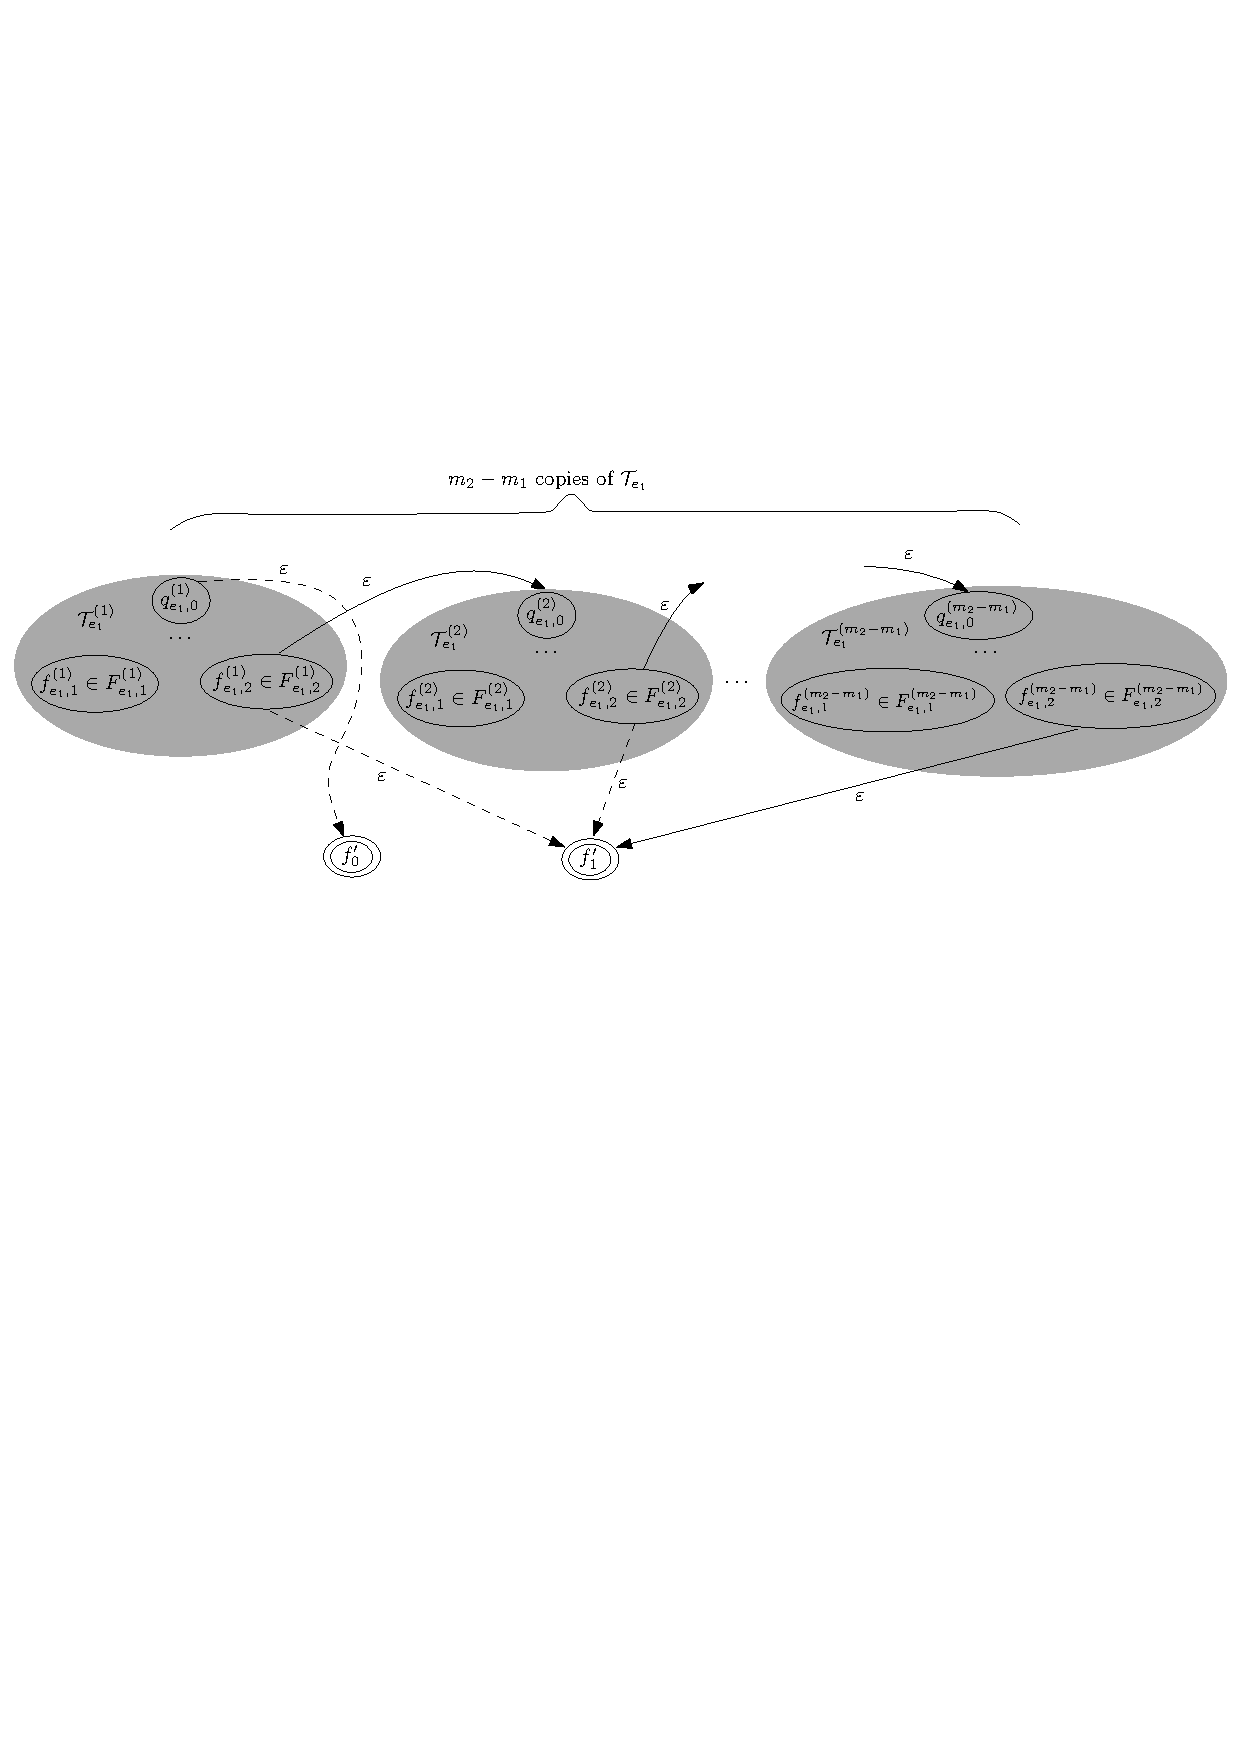
\includegraphics[width = 0.8\textwidth]{reg2pfa-4.pdf}
	\caption{The PSST $\cT^{\{1,m_2-m_1\}}_{e_1}$}
	\label{fig-reg2pfa-4}
\end{figure}  

Finally, we construct $\cT_e$ from $\cT^{\{m_1\}}_{e_1} \concat \cT^{\{1,m_2-m_1\}}_{e_1}$, the concatenation of $\cT^{\{m_1\}}_{e_1}$ and $\cT^{\{1,m_2-m_1\}}_{e_1}$, by adding a fresh state $q_{e,0}$, a string variable $x_e$, the $\varepsilon$-transition $\tau_e(q_{e,0}) = ((q_{e_1,0});())$ (assuming that $q_{e_1,0}$ is the initial state of $\cT^{\{m_1\}}_{e_1}$),  and the assignments $E_e(q_{e_0}, \varepsilon, q_{e_1,0})(x_e) = \varepsilon$, as well as $E_e(p, a, q)(x_e) = x_e a$ for each transition $(p, a, q)$ in  $\cT^{\{m_1\}}_{e_1} \concat \cT^{\{1,m_2-m_1\}}_{e_1}$.

%%%%%%%%%%%%%%%%%%%%%%%%%%%%%%%%%%%%%%%%%%%%%%%%%%%%%%%%%%%%%%%%%%%%%%%%%%%%%%%%%%%%%%%%%%%%%%%%%%%%%
\paragraph{Case $e = [e_1^{\{m_1,m_2\}?}]$ for $1 \le m_1 < m_2$ (see Figure~\ref{fig-reg2pfa-5})} Then $\cT_e$ is constructed as the concatenation of $\cT^{\{m_1\}}_{e_1}$ and $\cT^{\{1,m_2-m_1\}?}_{e_1}$, where $\cT^{\{1,m_2-m_1\}?}_{e_1}$ is illustrated in Figure~\ref{fig-reg2pfa-5}, which is the same as $\cT^{\{1,m_2-m_1\}}_{e_1}$ in Figure~\ref{fig-reg2pfa-4}, except that the priorities of the $\varepsilon$-transition from $q^{(1)}_{e_1,0}$ to $f^\prime_0$ has the highest priority and  the priorities of the $\varepsilon$-transitions out of each $f^{(i)}_{e_1,2} \in F^{(i)}_{e_1,2}$ to $f^\prime_1$ are swapped.
\begin{figure}[ht]
	\centering
	%\rule{\linewidth}{0cm}
	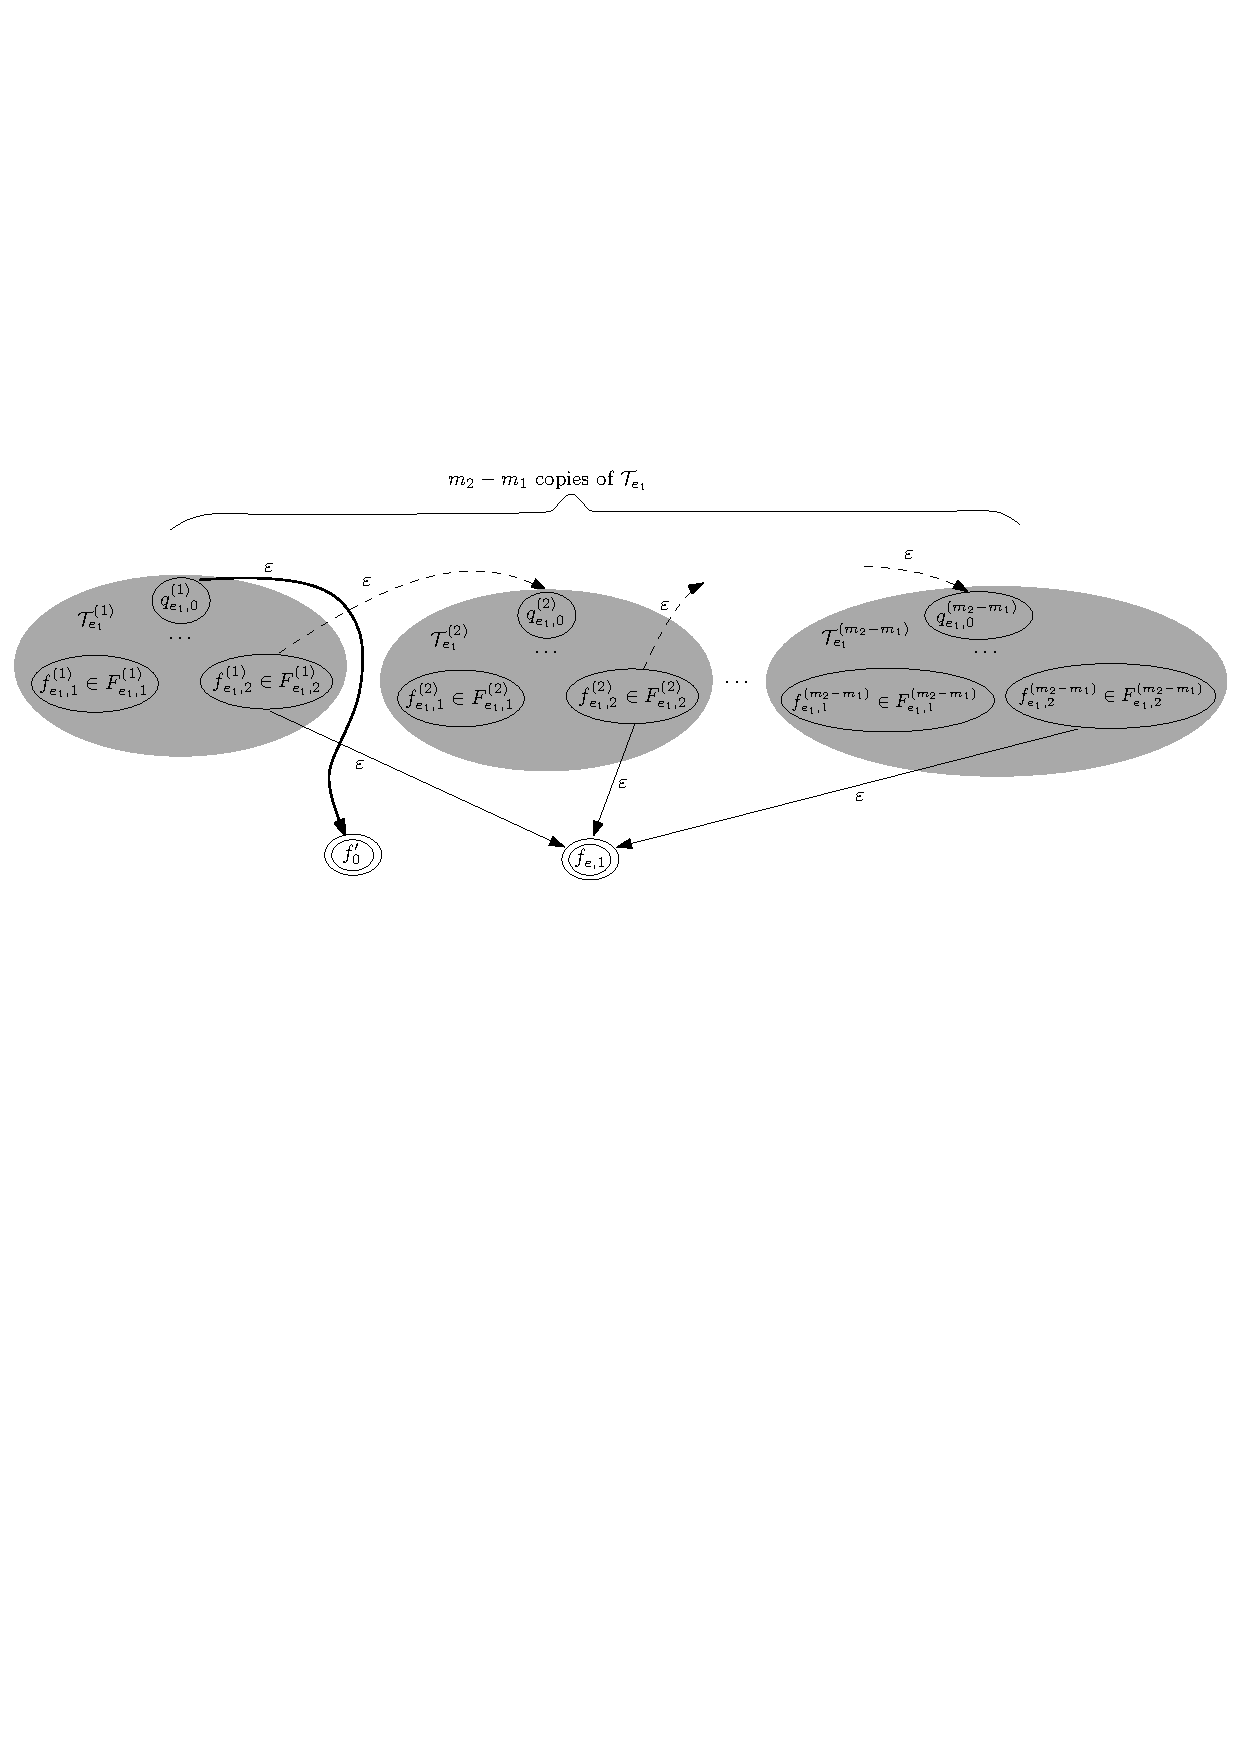
\includegraphics[width = 0.8\textwidth]{reg2pfa-5.pdf}
	\caption{The PSST $\cT^{\{1,m_2-m_1\}?}_{e_1}$}
	\label{fig-reg2pfa-5}
\end{figure} 

%%%%%%%%%%%%%%%%%%%%%%%%%%%%%%%%%%%%%%%%%%%%%%%%%%%%%
%%%%%%%%%%%%%%%%%%%%%%%%%%%%%%%%%%%%%%%%%%%%%%%%%%%%%
\OMIT{
\subsection{Backward Reasoning in the Motivating Example}\label{app-br-mot-exmp}

The path feasibility problem of the program in Equation~(\ref{eqn:exmp}) is solved by ``backward'' reasoning as follows:
\begin{itemize}
    \item At first, we compute the pre-image of $(\Aut_{\scriptsize\mbox{\tt /\^{}0\textbackslash d+.*|.*{\scriptsize\textbackslash}.\textbackslash d*0\$/}})$ under the concatenation $\concat$, which is a finite union of products of regular languages, remove $\tt result2 := integer \concat ``." \concat fractional$, select one disjunct of the union, say $(\Aut'_1, \Aut'_2)$, add the assertion $\ASSERT{\tt integer \in \Aut'_1};\ASSERT{\tt fractional \in \Aut'_2}$, resulting into the following program,
        \begin{eqnarray}\label{eqn:exmp-2}
            & & \ASSERT{\tt decimal \in \Aut_{decimalReg}};\nonumber \\
            & & \tt integer  := \tt  \cT_{\tt replace(\mbox{\scriptsize \tt /\^{}0+/, ""})}(\cT_{\tt extract_{decimalReg,1}}(decimal));\nonumber \\
            & & \tt fractional  := \tt  \cT_{\scriptsize\tt replace(\mbox{\tt /0+\$/, ""})}(\cT_{\tt extract_{decimalReg,2}}(decimal));\nonumber \\
            &&  \ASSERT{\tt integer \in \Aut_{\scriptsize\mbox{\tt.+}}};
            %\nonumber\\
            %&&  \tt result1 := integer;\nonumber\\
            \ASSERT{\tt fractional \in \Aut_{\scriptsize\mbox{\tt.+}}}; \nonumber\\
            % && \tt result2 := integer \concat ``." \concat fractional; \nonumber\\
            && \ASSERT{\tt result2 \in \Aut_{\scriptsize\mbox{\tt /\^{}0\textbackslash d+.*|.*{\scriptsize\textbackslash}.\textbackslash d*0\$/}}}; \nonumber\\
            && \ASSERT{\tt integer \in \Aut'_1};\ASSERT{\tt fractional \in \Aut'_2};
        \end{eqnarray}
        %
    \item Next, we compute the pre-image of $\Aut'_2$ under $\cT_{\tt extract_{decimalReg,2}}$ (see Lemma~\ref{lem:psst_preimage}), denoted by $\cB_1$, then the pre-image of $\Lang(\cB_1)$ under $\cT_{\tt replace(\mbox{\scriptsize \tt /0+\$/, ""})}$, denoted by $\cB'_1$. Similarly, we compute the pre-image of $\Aut_{\scriptsize\mbox{\tt.+}}$ under $\cT_{\tt extract_{decimalReg,2}}$ as well as $\cT_{\tt replace(\mbox{\scriptsize \tt /\^{}0+/, ""})}$,  and obtain a finite automaton $\cB'_2$. Moreover, we remove the assignment statement for  $\tt fractional$, and add the assertions $\ASSERT{\tt decimal \in \cB'_1}; \ASSERT{\tt decimal \in \cB'_2}$. Finally, we compute the pre-images of $\Aut'_1$ and $\Aut_{\scriptsize\mbox{\tt.+}}$ under $\cT_{\tt extract_{decimalReg, 1}}$ as well as $\cT_{\tt replace(\mbox{\scriptsize \tt /\^{}0+/, ""})}$, and obtain finite automata $\cC'_1$ and $\cC'_2$ respectively. Then we remove the assignment for {\tt integer}, and add $\ASSERT{\tt decimal \in \cC'_1};\ASSERT{\tt decimal \in \cC'_2}$. In the end, we get the following program containing no assignment statements,
        \begin{eqnarray}\label{eqn:exmp-3}
            & & \ASSERT{\tt decimal \in \Aut_{decimalReg}};\nonumber \\
            %& & \tt integer  := \tt  \cT_{\tt replace(\mbox{\scriptsize \tt /\^{}0+/, ""})}(\cT_{\tt match_{decimalReg,1}}(decimal));\nonumber \\
            %& & \tt fractional  := \tt  \cT_{\scriptsize\tt replace(\mbox{\tt /\^{}0+/, ""})}(\cT_{\tt match_{decimalReg,2}}(decimal));\nonumber \\
            &&  \ASSERT{\tt integer \in \Aut_{\scriptsize\mbox{\tt.+}}};
            %\nonumber\\
            %&&  \tt result1 := integer;\nonumber\\
            \ASSERT{\tt fractional \in \Aut_{\scriptsize\mbox{\tt.+}}}; \nonumber\\
            % && \tt result2 := integer \concat ``." \concat fractional; \nonumber\\
            && \ASSERT{\tt result2 \in \Aut_{\scriptsize\mbox{\tt /\^{}0\textbackslash d+.*|.*{\scriptsize\textbackslash}.\textbackslash d*0\$/}}}; \nonumber\\
            && \ASSERT{\tt integer \in \Aut'_1};\ASSERT{\tt fractional \in \Aut'_2}; \nonumber\\
            && \ASSERT{\tt decimal \in \cB'_1};\ASSERT{\tt decimal \in \cB'_2}; \nonumber\\
            && \ASSERT{\tt decimal \in \cC'_1};\ASSERT{\tt decimal \in \cC'_2};
        \end{eqnarray}
        %
    \item Finally, we check the nonemptiness of the intersection of the regular languages for the input variable $\tt decimal$, namely, $\Lang(\Aut_{\tt decimalReg})$, $\Lang(\cB'_1)$, $\Lang(\cB'_2)$, $\Lang(\cC'_1)$, and $\Lang(\cC'_2)$. If the intersection is nonempty, then the invariant property does \emph{not} hold.
\end{itemize}


\subsection{Undecidability of $\strline$}

\noindent {\bf Proposition~\ref{prop-und}}.
{\it The path feasibility problem of $\strline$ is undecidable}.

\begin{proof}
    The proof of Proposition~\ref{prop-und} is obtained by an encoding of post correspondence problem (PCP).
    Let $\Sigma$ be a finite alphabet such that $\# \not\in \Sigma$ and $[n] \cap \Sigma = \emptyset$, $(u_i, v_i)_{i \in [n]}$ be a PCP instance with $u_i, v_i \in \Sigma^\ast$. A solution of the PCP instance is a string $i_1 \cdots i_m$ with $i_j \in [n]$ for every $j \in [m]$ such that $u_{i_1} \cdots u_{i_m} = v_{i_1} \cdots v_{i_m}$. We will use $\replaceall$ to encode the generation of the strings $u_{i_1} \cdots u_{i_m}$ and $v_{i_1} \cdots v_{i_m}$ from $i_1 \cdots i_m$, then use a regular expression with  capturing groups and backreferences to verify the equality of $u_{i_1} \cdots u_{i_m}$ and $v_{i_1} \cdots v_{i_m}$. Specifically, the PCP instance is encoded by the following $\strline$ program,
    \[
        \begin{array}{l}
            \ASSERT{x_0 \in \{1, \cdots, n\}^+}; \\
            x_1 := \replaceall_{1, u_1}(x_0); \cdots; x_n:=\replaceall_{n, u_n}(x_{n-1}); \\
            y_1:=\replaceall_{1, v_1}(x_0); \cdots; y_n:=\replaceall_{n, u_n}(y_{n-1});\\
            z:= x_n \# y_n; \ASSERT{z \in (\Sigma^+)\#\$1}.
        \end{array}
    \]
    Note that the above program uses backreferences in assertion statements.
    We can achieve the same reduction by replacing $\ASSERT{z \in (\Sigma^+)\#\$1}$ in the above program with $z':= \replace(\Sigma^+\#\$1, \top); \ASSERT{z' \in \top}$, where $\top \not \in \Sigma$. Note that the program resulted from the replacement uses backreferences only in the pattern parameter of the $\replace$ function.
\end{proof}
}
%%%%%%%%%%%%%%%%%%%%%%%%%%%%%%%%%%%%%%%%%%%%%%%%%%%%%
%%%%%%%%%%%%%%%%%%%%%%%%%%%%%%%%%%%%%%%%%%%%%%%%%%%%%

% \subsection{Proof for Theorem \ref{theorem:regex_pnfa_equiv}}
%
% \label{proof:regex_pnfa_equiv}
%
% We restate the theorem here:
% \begin{theorem}
%   For any regular expression e, subexpression $e'$ of e, and $w \in L (e)$,
%   $m_{e', e} (w) = p_{e', e} (w)$
% \end{theorem}
%
% \begin{proof}
%   We first observe the fact that when $e' = e$, we have $m_{e', e} (w) =
%   p_{e', e} (w) = w$. Therefore, we suppose $e' \neq e$ in the following
%   argument.
%
%   We perform induction on $e$:
%   \begin{itemize}
%     \item The base case, when $e = \varepsilon$ or $e = a$, is routine and
%     trivial.
%
%     \item If $e = (e_1)$, then for any $w \in L (e)$, we have $w \in L (e_1)$,
%     and for any subexpression $e' \neq e$, $e'$ is also a subexpression of
%     $e_1$. By induction, \ $m_{e', e_1} (w) = p_{e', e_1} (w)$. Because $A_e =
%     A_{e_1}$, $p_{e', e_1} (w) = p_{e', e} (w)$. By definition of match tree,
%     we also have $m_{e', e_1} (w) = m_{e', e} (w)$. Thus $m_{e', e} (w) =
%     p_{e', e} (w)$.
%
%     \item If $e = e_1 + e_2$, then for any $w \in L (e)$, either $w \in L
%     (e_1)$ or $w \in L (e_2)$. Also, any subexpression $e' \neq e$ is a
%     subexpression of either $e_1$ or $e_2$.
%
%     If $w \in L (e_1)$, then if $e'$ is a subexpression of $e_2$, we have
%     $m_{e', e} (w) = p_{e', e} (w) = \emptyset$, otherwise by induction we
%     have $m_{e', e_1} (w) = p_{e', e_1} (w)$. Suppose $p = q_0 a_1 q_1
%     \ldots a_m q_m$ is the accepting run of $A_{e_1}$, then by definition
%     of $A_e$, we know p is also the accepting run of $A_e$, thus $p_{e', e_1}
%     (w) = p_{e', e} (w)$. By definition of match tree, we have $m_{e', e_1}
%     (w) = m_{e', e} (w)$. Thus $m_{e', e} (w) = p_{e', e} (w)$.
%
%     Similarly, when $w \in L (e_2)$, we also have $m_{e', e} (w) = p_{e', e}
%     (w)$.
%
%     \item If $e = e_1 e_2$, then for any $w \in L (e)$, suppose $w = w_1 w_2$
%     such that $C (m_e (w)) = (w_1, e_1) (w_2, e_2)$.
%
%     Assuming $p = q_0 a_1 q_1 \ldots a_m q_m$ is the accepting run
%     of $A_e$ on w, and $w_1 = a_1 \ldots a_i$, $w_2 = a_{i + 1}
%     \ldots a_m$, we know $q_0 a_1 q_1 \ldots a_i q_i$ is the
%     accepting run of $A_{e_1}$ on $w_1$. If not, suppose the accepting run of
%     $A_{e_1}$ on $w_1$ is $q_0 a_1' q_1' \ldots a_i' q_i'$ instead,
%     then by definition of $A_e$, another run of $A_e$ on
%     w, $q_0 a_1' q_1' \ldots a_i' q_i'
%     a_{i + 1} q_{i + 1} \ldots a_m q_m$, is of higher priority than p, which leads to contradiction.
%     Similarly, we know $q_0 a_{i + 1} q_{i + 1} \ldots a_m q_m$ is
%     the accepting run of $A_{e_2}$ on $w_2$.
%
%     If $e'$ is a subexpression of $e_1$, then by induction, $m_{e', e_1} (w_1)
%     = p_{e', e_1} (w_1)$. By definition of match tree, $e'$ cannot occur in
%     the subtree $(w_2, e_2)$, thus we have $m_{e', e_1} (w_1) = m_{e', e}
%     (w)$. Because the maximal $e'$-matches in p only occur in $q_0 a_1
%     q_1 \ldots a_i q_i$, we also have $p_{e', e_1} (w_1) = p_{e', e}
%     (w)$. Thus $m_{e', e} (w) = p_{e', e} (w)$.
%
%     Similarly when $e'$ is a subexpression of $e_2$, we have $m_{e', e} (w) =
%     p_{e', e} (w)$.
%
%     \item If $e = e_1^{\ast}$, then for any $w \in L (e)$, if $w =
%     \varepsilon$ it is obvious that $m_{e', e} (w) = p_{e', e} (w) =
%     \emptyset$ for any $e'$. Otherwise, suppose $w = w_1 \ldots w_n$ such that
%     $C (m_e (w)) = (w_1, e_1) \ldots (w_n, e_1)$.
%
%     Assuming $p = q_0 a_1 q_1 \ldots a_m q_m$ is the accepting run
%     of $A_e$ on w, $w_1 = a_1 \ldots a_{i_1}$, $w_2 = a_{i_1 +
%     1} \ldots a_{i_2}$ .etc, and $w_n = a_{i_{m - 1} + 1} \ldots
%     a_m$, we know $p_k = q_0 a_{i_{k - 1} + 1} q_{i_{k - 1} + 1}
%     \ldots a_{i_k} q_{i_k}$ is the accepting run of $A_{e_1}$ on
%     $w_k$. The proof is similar to the one above when $e = e_1 e_2$, and we
%     will omit it for simplicity.
%
%     For any subexpression $e'$ of $e_1$, by induction, we have $m_{e', e_1}
%     (w_k) = p_{e', e_1} (w_k)$ for all $k \in [n]$. By definition of match
%     tree, we have $m_{e', e} (w) = m_{e', e_1} (w_1) \ldots m_{e', e_1}
%     (w_n)$. Because all the maximal $e'$-matches in p only occur in $p_k$ for
%     some $k \in [n]$ (that is, all the states in a $e'$-matches occur in the
%     same segment of $p$), we also have $p_{e', e} (w) = p_{e', e_1} (w_1)
%     \ldots p_{e', e_1} (w_n)$. Thus $m_{e', e} (w) = p_{e', e} (w)$.
%   \end{itemize}
% \end{proof}


%======================================================

\subsection{From $\extract$, $\replace$ and $\replaceall$ to PSSTs}\label{appendix:sec-extract-replace-to-psst}

\noindent{\bf Lemma~\ref{lem-str-fun-to-psst}}.
    The satisfiability of $\strline$ reduces to the satisfiability of boolean combinations of formulas of the form $z=x \concat y$, $y=\cT(x)$, and $x \in \cA$, where $\cT$ is a PSST and $\cA$ is an FA.

    The proof is in two steps: first we remove $\$0$, $\refbefore$, and $\refafter$, then we encode the remaining string functions with PSSTs.

    \subsubsection{Removing Special References}


    The first step in our proof is to remove the special references $\$0$, $\refbefore$, and $\refafter$ from the replacement strings.
    These can be replaced in a series of steps, leaving only PSST transductions and replacement strings with only simple references ($\$i$).
    We will just consider $\replaceall$ as $\replace$ is almost identical.

    First, to remove $\$0$, suppose we have a statement
    $y := \replaceall_{\pat, \rep}(x)$
    with $\$0$ in $\rep$.
    We simply substitute
    $y := \replaceall_{\pat', \rep'}(x)$
    where
        $\pat' = (\pat)$, and
        $\rep' = \rep[\$1 / \$0, \$2 / \$1, \ldots, \$(k+1) / \$k]$.
    That is, we make the complete match an explicit (first) capture, which shifts the indexes of the remaining capture groups by 1.

    Now suppose we have a statement
    $y := \replaceall_{\pat, \rep}(x)$
    with $\refbefore$ or $\refafter$ in $\rep$.
    We replace it with the following statements, explained below, where
    $y_1, \ldots, y_5$
    are fresh variables.
    \[
        \begin{array}{l}
            y_1 := \replaceall_{(\pat), \langle\$1\rangle}(x); \\
            y_2 := \psst_{\langle}(y_1); \\
            y_3 := \psst_{\mathrm{rev}}(y_2); \\
            y_4 := \psst_{\rangle}(y_3); \\
            y_5 := \psst_{\mathrm{rev}}(y_4); \\
            y := \replaceall_{\pat', \rep'}(y_5)
        \end{array}
    \]

    The first step is to mark the matched parts of the string with $\langle$ and $\rangle$ brackets (where $\langle$ and $\rangle$ are not part of the main alphabet).
    This is achieved by the first $\replaceall$.

    Next, we use a PSST $\psst_{\langle}$ that passes over the marked word.
    This is a copyful PSST that simply stores the word read so far into a variable $X$, except for the $\langle$ and $\rangle$ characters.
    It also has an output variable $O$, to which it also copies each character directly, except $\langle$.
    When it encounters $\langle$ it appends to $O$ the string
    $\langle X \langle$.
    That is, it puts the entire string preceding each $\langle$ into the output, surrounded by $\langle$ at the start and end.
    This is copyful since $X$ will be copied to both $X$ and $O$ in this step.
    For example, suppose the input string were
    $a b \langle c \rangle d \langle e \rangle f$,
    the output of $\psst_\langle$ would be
    $a b \langle \underline{a b} \langle c \rangle d \langle \underline{a b c d} \langle e \rangle f$.
    We have underlined the strings inserted for readability.

    The next step is to do the same for $\rangle$.
    To achieve this we first reverse the string so that a PSST can read the end of the string first.
    A similar transduction to $\psst_\langle$ is performed before the string is reversed again.
    In our example the resulting string is
    $a b \langle \underline{a b} \langle c \rangle \underline{d e f} \rangle d \langle \underline{a b c d} \langle e \rangle \underline{f} \rangle f$.

    Finally, we have
    $y := \replaceall_{\pat', \rep'}(y_5)$
    where
    $\pat' =
         \langle (\Sigma^{*?}) \langle
         \pat
         \rangle (\Sigma^{*?}) \rangle$, and
    \[
        \rep' = \rep[
            \$1 / \refbefore,
            \$2 / \$1,
            \ldots
            \$(k+1) / \$k,
            \$(k+2) / \refafter
        ] \ .
    \]
    That is, by inserting the preceding and succeeding text directly next to each match, we can use simple references $\$i$ instead of $\refbefore$ and $\refafter$.

    \subsubsection{Encoding string functions as PSSTs}

    Once $\$0$, $\refbefore$, and $\refafter$ are removed from the replacement strings, then the string functions can be replaced by PSSTs.

    \begin{lemma}
        For each string function $f = \extract_{i,e}$, $\replace_{\pat, \rep}$, or $\replaceall_{\pat, \rep}$ without $\refbefore$ or $\refafter$ in the replacements strings, a PSST $\cT_f$ can be constructed such that
        $$\cR_{f} = \{(w, w') \mid w'= f(w)\}.$$
    \end{lemma}
    \begin{proof}
    The $\extract_{i,e}$ can function be defined by a PSST $\cT_{i,e}$ obtained from the PSST $\cT_e$ (see Section~\ref{sect:regextopsst}) by removing all the string variables, except the string variable $x_{e'}$, where $e'$ is the subexpression of $e$ corresponding to the $i$th capturing group,  and setting the output expression of the final states as $x_{e'}$.

%%%%%%%%%%%%%%%%%%%%%%%%%%%%%%%%%%%%%%%%%
%%%%%%%%%%%%%%%%%%%%%%%%%%%%%%%%%%%%%%%%%
        Let $e'$ be the subexpression corresponding to the $i$-th capturing group of $e$. In particular, if $i=0$, then $e' = e$.
        Suppose $\cA_e = (Q, \Sigma, \delta, \tau, q_0, f_0)$, and ${\sf Sub}_{e'}[\cA_e]$ is any isomorphic copy of $\cA_{e'}$ in $\cA_e$.

        Intuitively, $\cT_{\extract_{i,e}}$ (see Fig.~\ref{fig-psst-extract})
        \begin{itemize}
            \item uses a string variable $x$ to store the value of the $i$th capturing group,
            \item initially assigns $\nullchar$ to $x$ to denote the fact that the capturing group is not matched yet,
            \item then simulates $\cA_e$ and stores letters into $x$ when applying the transitions in ${\sf Sub}_{e'}[\cA_e]$,
            \item finally outputs the value of $x$ when $\cA_e$ accepts.
        \end{itemize}

        \begin{figure}[ht]
            \centering
            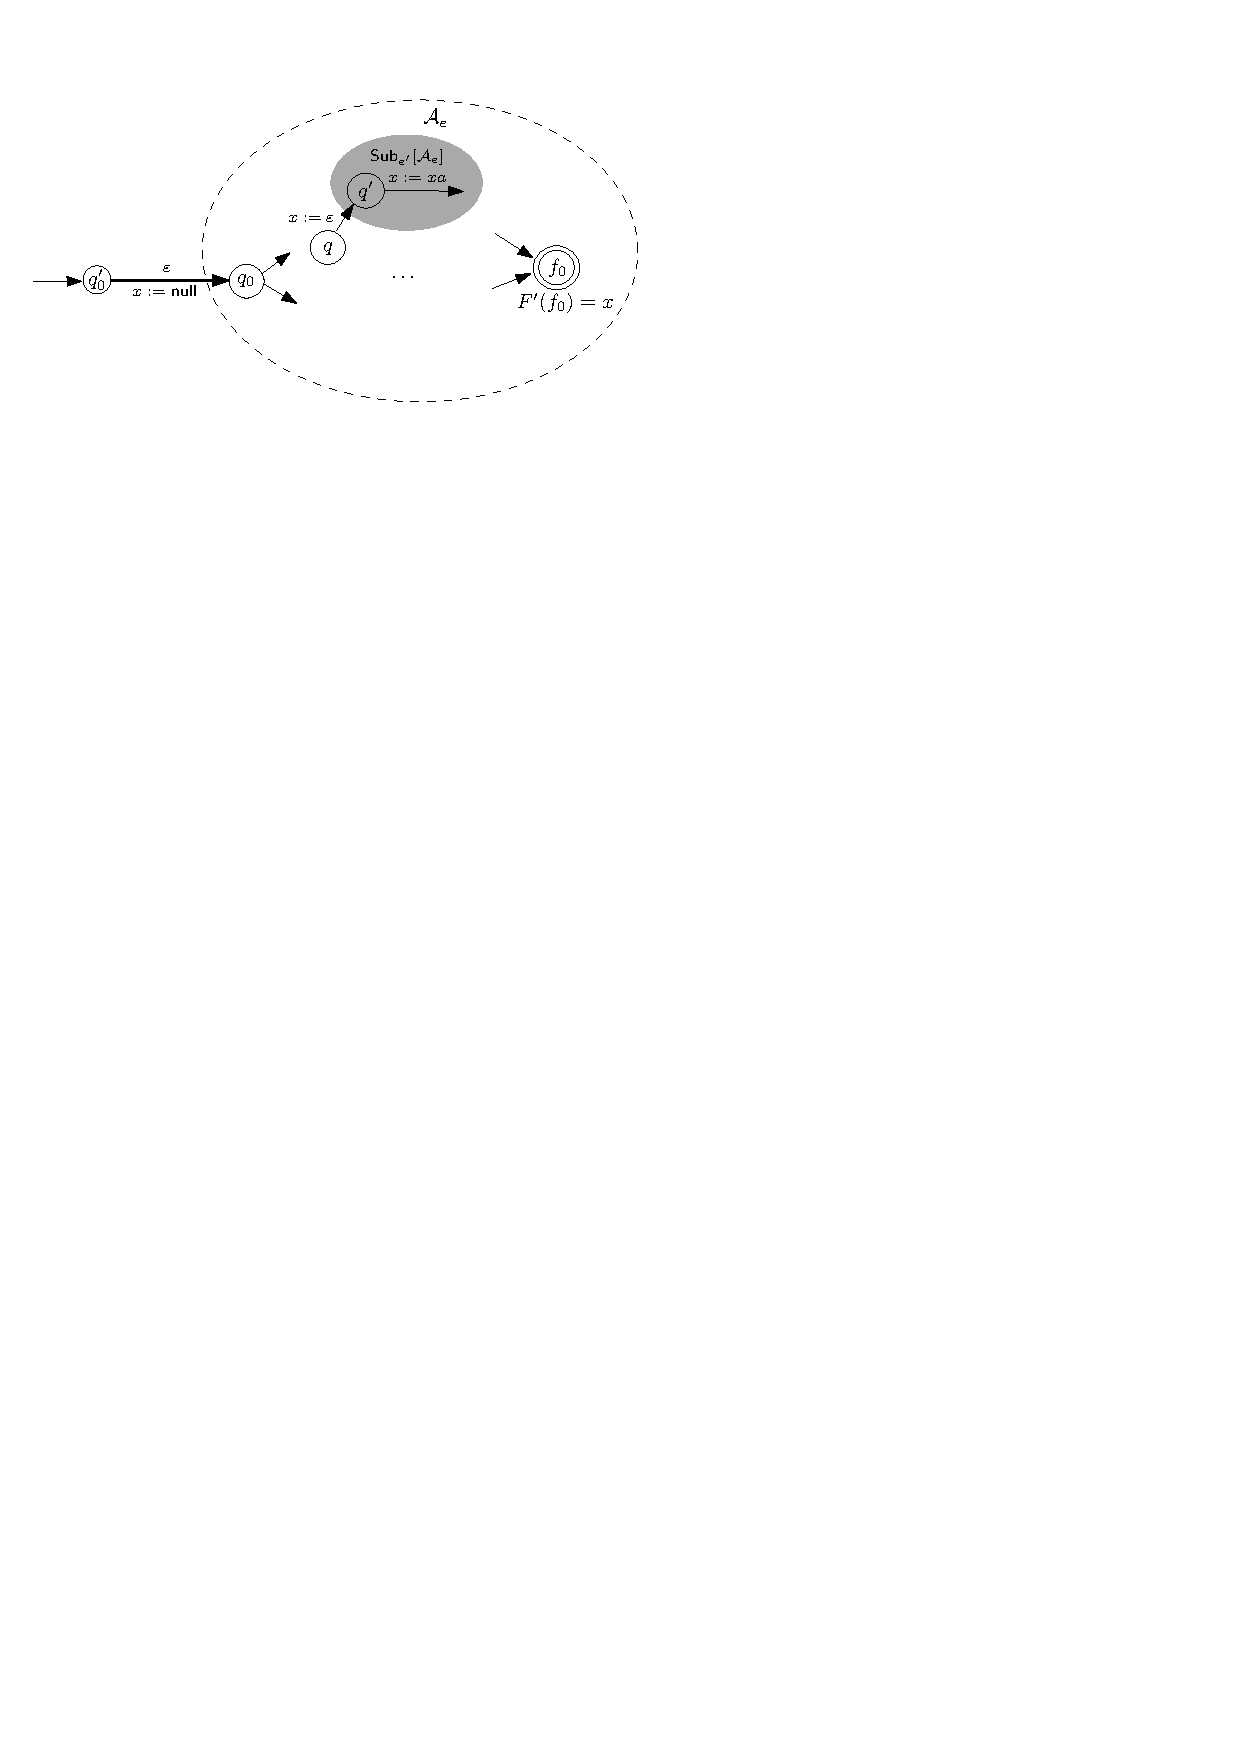
\includegraphics[width = 0.6\textwidth]{psst-extract.pdf}
            \caption{The PSST $\cT_{\extract_{i,e}}$}
            \label{fig-psst-extract}
        \end{figure}

        Formally, $\cT_{\extract_{i,e}} = (Q \cup \{q'_0\}, \Sigma, X, \delta', \tau', E', q'_0, F')$, where
        \begin{itemize}
            \item $q'_0 \not \in Q$,
                %
            \item $X = \{x\}$,
                %
            \item $F'(f_0)= x$ and $F'(p)$ is undefined for all the other states $p \in Q  \cup \{q'_0\}$,
                %
            \item $\delta'$ and $\tau'$ are defined as follows,
                \begin{itemize}
                    \item $\tau'(q'_0) = ((q_0); ())$,
                        %
                    \item $\delta'$ includes all the transitions in $\delta$,
                        %
                    \item $\tau'$ includes all the transitions in $\tau$,
                        %
                \end{itemize}
                %
            \item $E'$ is defined as follows,
                \begin{itemize}
                    \item $E'(q'_0, \varepsilon, q_0)(x) = \nullchar$,
                        %
                    \item for each transition $(q, a, q')$ in ${\sf Sub}_{e'}[\cA_e]$ such that $q$ is the inital state of ${\sf Sub}_{e'}[\cA_e]$(Note in this case, the construction in Proposition \ref{prop-rwre-to-pfa} ensures $a$ equals $\varepsilon$), $E'(q, a, q')(x) = \varepsilon$,
                    \item for each other transition $(q, a, q')$ in ${\sf Sub}_{e'}[\cA_e]$, $E'(q, a, q')(x) = x a$,
                        %

                        %
                    \item for all the other transitions $t$ of $\cA_e$, $E'(t)(x) = x$.
                \end{itemize}
                %
        \end{itemize}
%%%%%%%%%%%%%%%%%%%%%%%%%%%%%%%%%%%%%%%%%
%%%%%%%%%%%%%%%%%%%%%%%%%%%%%%%%%%%%%%%%%

        Next, we give the construction of the PSST for $\replaceall_{\pat, \rep}$ where all the references in $\rep$ are of the form $\$i$.
        Recall $\rep = w_1 \$i_1 w_2 \cdots w_k \$i_k w_{k+1}$.
        Let $\cT_{\replaceall_{\pat, \rep}} = (Q_\pat \cup \{q'_0\}$, $\Sigma$, $X'$, $\delta'$, $\tau', E', q'_0, F')$ where
        \begin{itemize}
            \item $q'_0 \not \in Q_\pat$,

            \item  $X' = \{x_0\} \cup X_\pat$,
                %
            \item $F'(q'_0) = x_0$, and $F'(q')$ is undefined for every $q' \in Q_\pat$,
                %
            \item $\delta'$ comprises the transitions in $\delta_\pat$, and the transition $\delta'(q'_0, a) = (q'_0)$ for $a \in \Sigma$,

            \item  $\tau'$ comprises the transitions in $\tau_\pat$, the transitions $\tau'(q'_0) = ((q_{\pat, 0}); ())$, $\tau'(f_{\pat, 1}) = ((q_{\pat, 0}); ())$ and $\tau'(f_{\pat, 2}) = ((q_{\pat, 0}); ())$ for $f_{\pat, 1} \in F_{\pat, 1}$ and $f_{\pat, 2} \in F_{\pat, 2}$,
                \begin{itemize}
                    \item $\delta'(q'_0, a) = (q'_0)$ for every $a \in \Sigma$, and $\tau'(q'_0) = ((q_0); ())$,
                        %
                    \item for every $q \in Q \setminus \{f_0\}$ and $a \in \Sigma$, $\delta'(q, a) = \delta(q, a)$ and $\tau'(q) = \tau(q)$,
                        %
                    \item $\delta'(f_0, a) = ()$ for every $a \in \Sigma$ and $\tau'(f_0) = ((q'_0); ())$,
                \end{itemize}
                %
            \item $E'$ inherits $E_\pat$, and includes the assignments $E'(q'_0, a, q'_0)(x_0)  = x_0 a$ for $a \in \Sigma$, $E'(f, \varepsilon, q'_0) (x_0) = x_0\rep[x_{e'_{i_1}}/\$i_1, \ldots, x_{e'_{i_k}}/i_k]$ and $E'(f, \varepsilon, q'_0) (x) = \nullchar$ for every  $f \in F_{\pat,1} \cup F_{\pat, 2}$ and $x \in X_\pat$.
                \begin{itemize}
                    \item for every transition $(q, a, q')$ with $a \in \Sigma^\varepsilon$ in $\cA_\pat$, $E(q, a, q')(x_0) = x_0$,
                        %
                    \item for every transition $(q, a, q')$ with $a \in \Sigma^\varepsilon$ and every $j \in [k]$,  if $(q, a, q')$ occurs in ${\sf Sub}_{e'_{i_j}}[\cA_\pat]$, then $E(q, a, q')(x_j) = x_ja$, otherwise, $E(q, a, q')(x_j) = x_j$,
                        %
                    \item  for every $a \in \Sigma$ and $j \in [k]$, $E(q'_0, a, q'_0)(x_0) = x_0a$ and $E(q'_0, a, q'_0)$$(x_j) = x_j$,
%
                    \item $E(q'_0, \varepsilon, q_0)(x_j) = x_j$ for every $j \in [k] \cup \{0\}$,
                        %
                    \item $E(f_0, \varepsilon, q'_0)(x_0) = x_0 \rep[x_1/\$i_1,\ldots, x_k/\$i_k]$, moreover, for every $j \in [k]$, $E(f_0, \varepsilon, q'_0)(x_j) = \varepsilon$, where $ \rep[x_1/\$i_1,\ldots, x_k/\$i_k]$ denotes the string term obtained from $\rep$ by replacing every occurrence of $\$i_1,\cdots, \$i_k$ with $x_1,\cdots,x_k$ respectively.
                        %
                \end{itemize}
                %
        \end{itemize}
        \end{proof}

        The construction of the PSST for $\replace_{\pat, \rep}$ is similar and illustrated in Fig.~\ref{fig-psst-replace}. The details are omitted.
        \begin{figure}[ht]
            \centering
            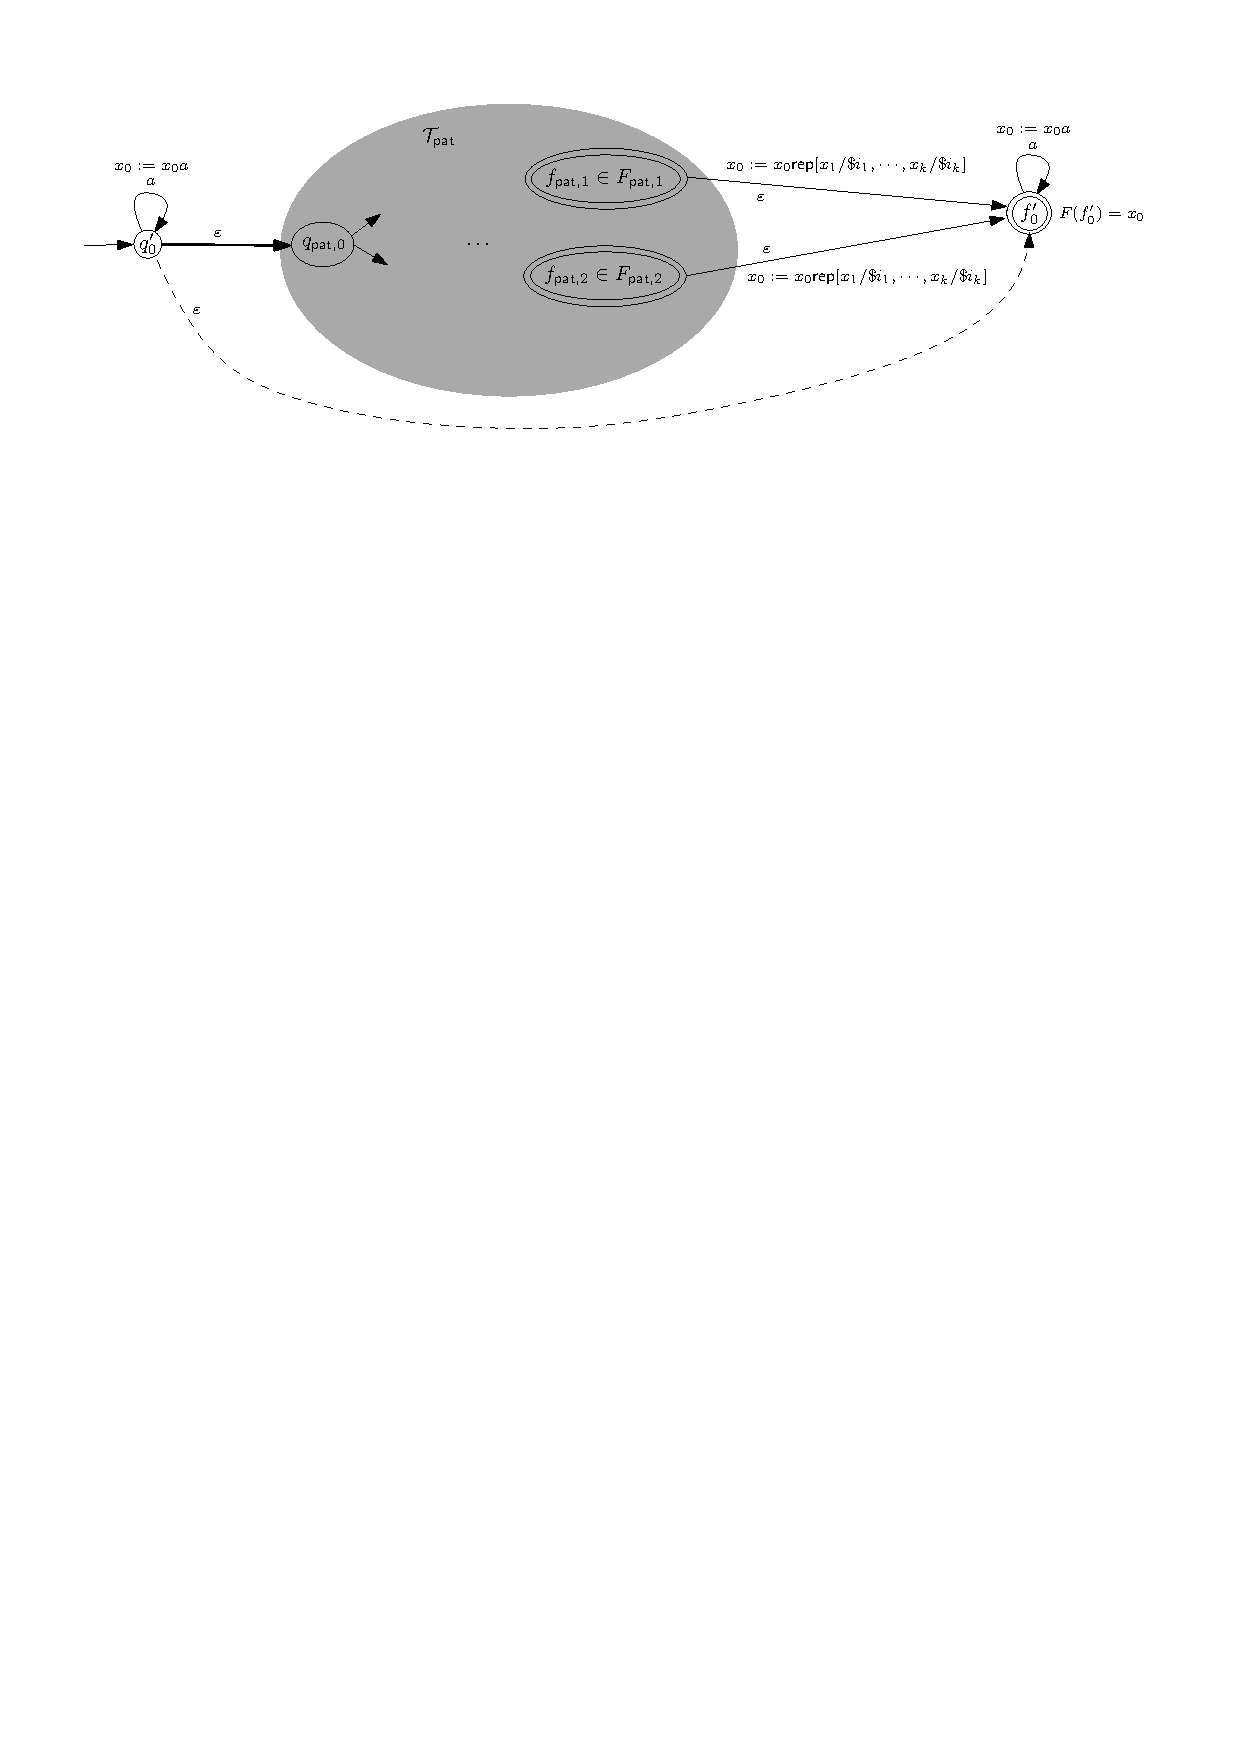
\includegraphics[width=\textwidth]{psst-replace.pdf}
            \caption{The PSST $\cT_{\replace_{\pat,\rep}}$}
            \label{fig-psst-replace}
        \end{figure}


%%%%%%%%%%%%%%%%%%%%%%%%%%%%%%%%%%%%%%
%%%%%%%%%%%%%%%%%%%%%%%%%%%%%%%%%%%%%%
\subsection{Proof of Lemma~\ref{lem:psst_preimage}}\label{app-pre-image}

%Construction of an FA $\cB$ for $\cR^{-1}_\cT(\Lang(\cA))$

\medskip

\noindent {\bf Lemma~\ref{lem:psst_preimage}}.
\emph{  Given a PSST $\psst = (Q_T, \Sigma$, $X$, $\delta_T$, $\tau_T$, $E_T$,  $q_{0, T}$, $F_T$) and an \FA{} $\Aut
  = (Q_A, \Sigma, \delta_A, q_{0, A}, F_A)$, we can compute an \FA{} $\cB = (Q_B,
  \Sigma, \delta_B, q_{0, B}, F_B)$ in exponential time  such that $\Lang(\cB) = \cR^{-1}_{\cT}(\Lang(\Aut))$.
}

\medskip

We prove Lemma~\ref{lem:psst_preimage} in the sequel.

        Let $\psst = (Q_T, \Sigma$, $X, \delta_T, \tau_T, E_T,  q_{0, T}, F_T)$ be a PSST  and $\Aut
        = (Q_A, \Sigma$, $\delta_A$, $q_{0, A}$, $F_A)$ be an \FA{}. Without loss of generality, we assume that $\Aut$ contains no $\varepsilon$-transitions. For convenience, we use $\cE(\tau_T)$ to denote $\{(q, q') \mid q' \in \tau_T(q)\}$. For convenience, for $a \in \Sigma$, we use $\delta^{(a)}_A$ to denote the  relation $\{(q, q') \mid (q, a, q') \in \delta_A\}$.

        To illustrate the intuition of the proof of Lemma~\ref{lem:psst_preimage}, let us start with the following natural idea of firstly constructing a PFA $\cB$ for the pre-image: $\cB$ simulates a run of $\psst$ on $w$, and, for each $x \in X$, records an $\Aut$-abstraction of the string stored in $x$, that is, the set of state pairs $(p, q) \in Q_A \times Q_A$ such that starting from $p$, $\Aut$ can reach $q$ after reading the string stored in $x$. Specifically, the states of $\cB$ are of the form $(q, \rho)$ with $q \in Q$ and $\rho \in (\cP(Q_A \times Q_A ))^{X}$. Moreover, the priorities of $\cB$ inherit those of $\psst$. The PFA $\cB$ is then transformed to an equivalent FA by simply dropping all priorities. We refer to this FA as $\cB'$.

        Nevertheless, it turns out that this construction is flawed: A string $w$ is in $\cR^{-1}_{\cT}(\Lang(\Aut))$ iff the (unique) accepting run of $\cT$ on $w$ produces an output $w'$ that is accepted by $\Aut$. However, a string $w$ is accepted by $\cB'$ iff \emph{there is a run of $\cT$ on $w$, not necessarily of the highest priority}, producing an output $w'$ that is accepted by $\Aut$. 
        

\OMIT{        
The following example illustrates the flaw of the construction above.

        \begin{example}
            \label{pre-image-count-examp}
            Let $\cT_{\tt extract_{decimalReg,1}}$ be the PSST in Fig.~\ref{fig-psst-exmp} and $\cA$ be the FA corresponding to the regular expression $\{1,\cdots,9\}^*$, specifically, $\cA= (\{p_0\}$, $\{0,\cdots,9\}$, $\delta_A$, $p_0, \{p_0\})$, where $\delta_A = \{(q_0, \ell, q_0) \mid \ell = 1, \cdots, 9\}$.
            %  in Figure~\ref{fig-pre-image-count-exmp}, that is,
            %\begin{itemize}
            %\item $\cT=(\{q_0, q_1, q_2\}, \{a,b,c\}, \{x_0\}, \delta_T, \tau_T, E_T, q_0, F_T)$, where $\delta_T(q_0, \sigma) = (q_0)$, $\delta_T(q_1, a) = (q_1)$, $\delta_T(q_2, \sigma) = (q_2)$, $\tau_T(q_0) = ((q_1); ())$, $\tau_T(q_1)=((q_0, q_2);())$, and $\tau_T(q_2)= ((); ())$, $E_T(q_0, \sigma, q_0) (x_0) = x_0 \sigma$, $E_T(q_1, \varepsilon, q_0) (x_0) = x_0 c$, $E_T(q_1, \varepsilon, q_2) (x_0) = x_0 c$, $E_T(q_2, \sigma, q_2) (x_0) = x_0 \sigma$, for $\sigma \in\{ a, b\}$. Moreover, $F_T(q_2)= x_0$;
            %
            %\item $\cA = (\{p_0\}, \{a,b,c\}, \delta_A, p_0, \{p_0\})$, where $\delta_A$ = $\{(p_0, \sigma, p_0)$ $\mid \sigma = b, c\}$.
            %\end{itemize}

            Let us consider $w = 10$. The accepting run of $\cT_{\tt extract_{decimalReg,1}}$ on $w$ is $q_0 \xrightarrow[x_1:=x_11]{1} q_1 \xrightarrow[x_1:=x_10]{0} q_1 \xrightarrow{\varepsilon} q_2 \xrightarrow{\varepsilon} q_3 \xrightarrow{\varepsilon} q_4 \xrightarrow{\varepsilon} q_5 \xrightarrow{\varepsilon} q_6$, producing an output $10 \not \in \Lang(\cA)$. Therefore, $10 \not \in \cR_\cT^{-1}(\Lang(\cA))$. Nevertheless, if we consider the FA $\cB'$ constructed from $\cT$ and $\cA$,  it turns out that $\cB'$ does accept $w$, witnessed by the run $(q_0, \{(p_0,p_0)\}) \xrightarrow{1} (q_1, \{(p_0, p_0)\}) \xrightarrow{\varepsilon} (q_2, \{(p_0, p_0)\}) \xrightarrow{\varepsilon}  (q_3, \{(p_0, p_0)\}) \xrightarrow{\varepsilon}  (q_4, \{(p_0, p_0)\}) \xrightarrow{\varepsilon}  (q_5, \{(p_0, p_0)\}) \xrightarrow{0}  (q_5, \{(p_0, p_0)\}) \xrightarrow{\varepsilon}  (q_6, \{(p_0, p_0)\})$, where $\{(p_0, p_0)\}$ is the $\cA$-abstraction of the strings $\varepsilon$ and $1$. On the other hand, the run of $\cB'$ corresponding to the accepting run of $\cT$ on $w$, i.e. $(q_0, \{(p_0, p_0)\}) \xrightarrow{1} (q_1, \{(p_0, p_0)\}) \xrightarrow{0} (q_1, \emptyset) \xrightarrow{\varepsilon}  (q_2, \emptyset) \xrightarrow{\varepsilon} (q_3, \emptyset) \xrightarrow{\varepsilon} (q_4, \emptyset) \xrightarrow{\varepsilon} (q_5, \emptyset) \xrightarrow{\varepsilon} (q_6, \emptyset)$, is not accepting, where $\{(p_0,p_0)\}$ is the $\cA$-abstraction of $\varepsilon$ as well as $1$, and $\emptyset$ is the $\cA$-abstraction of $10$.
        \end{example}
}

        %%%%%%%%%%%%%%%%%%%%%%%%%%%%%%
        %%%%%%%%%%%%%%%%%%%%%%%%%%%%%%
        \hide{
            \begin{example}
                \label{pre-image-count-examp}
                Let $\cT$ be the PSST and $\cA$ be the FA in Figure~\ref{fig-pre-image-count-exmp}, that is,
                \begin{itemize}
                    \item $\cT=(\{q_0, q_1, q_2\}, \{a,b,c\}, \{x_0\}, \delta_T, \tau_T, E_T, q_0, F_T)$, where $\delta_T(q_0, \sigma) = (q_0)$, $\delta_T(q_1, a) = (q_1)$, $\delta_T(q_2, \sigma) = (q_2)$, $\tau_T(q_0) = ((q_1); ())$, $\tau_T(q_1)=((q_0, q_2);())$, and $\tau_T(q_2)= ((); ())$, $E_T(q_0, \sigma, q_0) (x_0) = x_0 \sigma$, $E_T(q_1, \varepsilon, q_0) (x_0) = x_0 c$, $E_T(q_1, \varepsilon, q_2) (x_0) = x_0 c$, $E_T(q_2, \sigma, q_2) (x_0) = x_0 \sigma$, for $\sigma \in\{ a, b\}$. Moreover, $F_T(q_2)= x_0$;
                        %
                    \item $\cA = (\{p_0\}, \{a,b,c\}, \delta_A, p_0, \{p_0\})$, where $\delta_A$ = $\{(p_0, \sigma, p_0)$ $\mid \sigma = b, c\}$.
                \end{itemize}

                Let us consider $w = a$. The accepting run of $\cT$ on $w$ is $q_0 \xrightarrow{\varepsilon} q_1 \xrightarrow[x_0:=x_0c]{\varepsilon} q_0 \xrightarrow[x_0:=x_0a]{a} q_0 \xrightarrow{\varepsilon} q_1 \xrightarrow[x_0:=x_0c]{\varepsilon} q_2$, producing an output $cac \not \in \Lang(\cA)$. Therefore, $a \not \in \cR_\cT^{-1}(\Lang(\cA))$. Nevertheless, if we consider the FA $\cB'$ constructed from $\cT$ and $\cA$,  it turns out that $\cB'$ does accept $w$, witnessed by the run $(q_0, \{(p_0,p_0)\}) \xrightarrow{\varepsilon} (q_1, \{(p_0,p_0)\}) \xrightarrow{a} (q_1, \{(p_0, p_0)\}) \xrightarrow{\varepsilon}  (q_2, \{(p_0, p_0)\})$. On the other hand, the run of $\cB'$ corresponding to the accepting run of $\cT$ on $w$, i.e. $(q_0, \{(p_0,p_0)\}) \xrightarrow{\varepsilon} (q_1, \{(p_0,p_0)\}) \xrightarrow{\varepsilon} (q_0, \{(p_0, p_0)\}) \xrightarrow{a}  (q_0, \emptyset) \xrightarrow{\varepsilon} (q_1, \emptyset) \xrightarrow{\varepsilon} (q_2, \emptyset)$, is not accepting, where $\{(p_0,p_0)\}$ and $\emptyset$ are the $\cA$-abstractions of $x_0$.
            \end{example}

            \begin{figure}[ht]
                \centering
                %\rule{\linewidth}{0cm}
                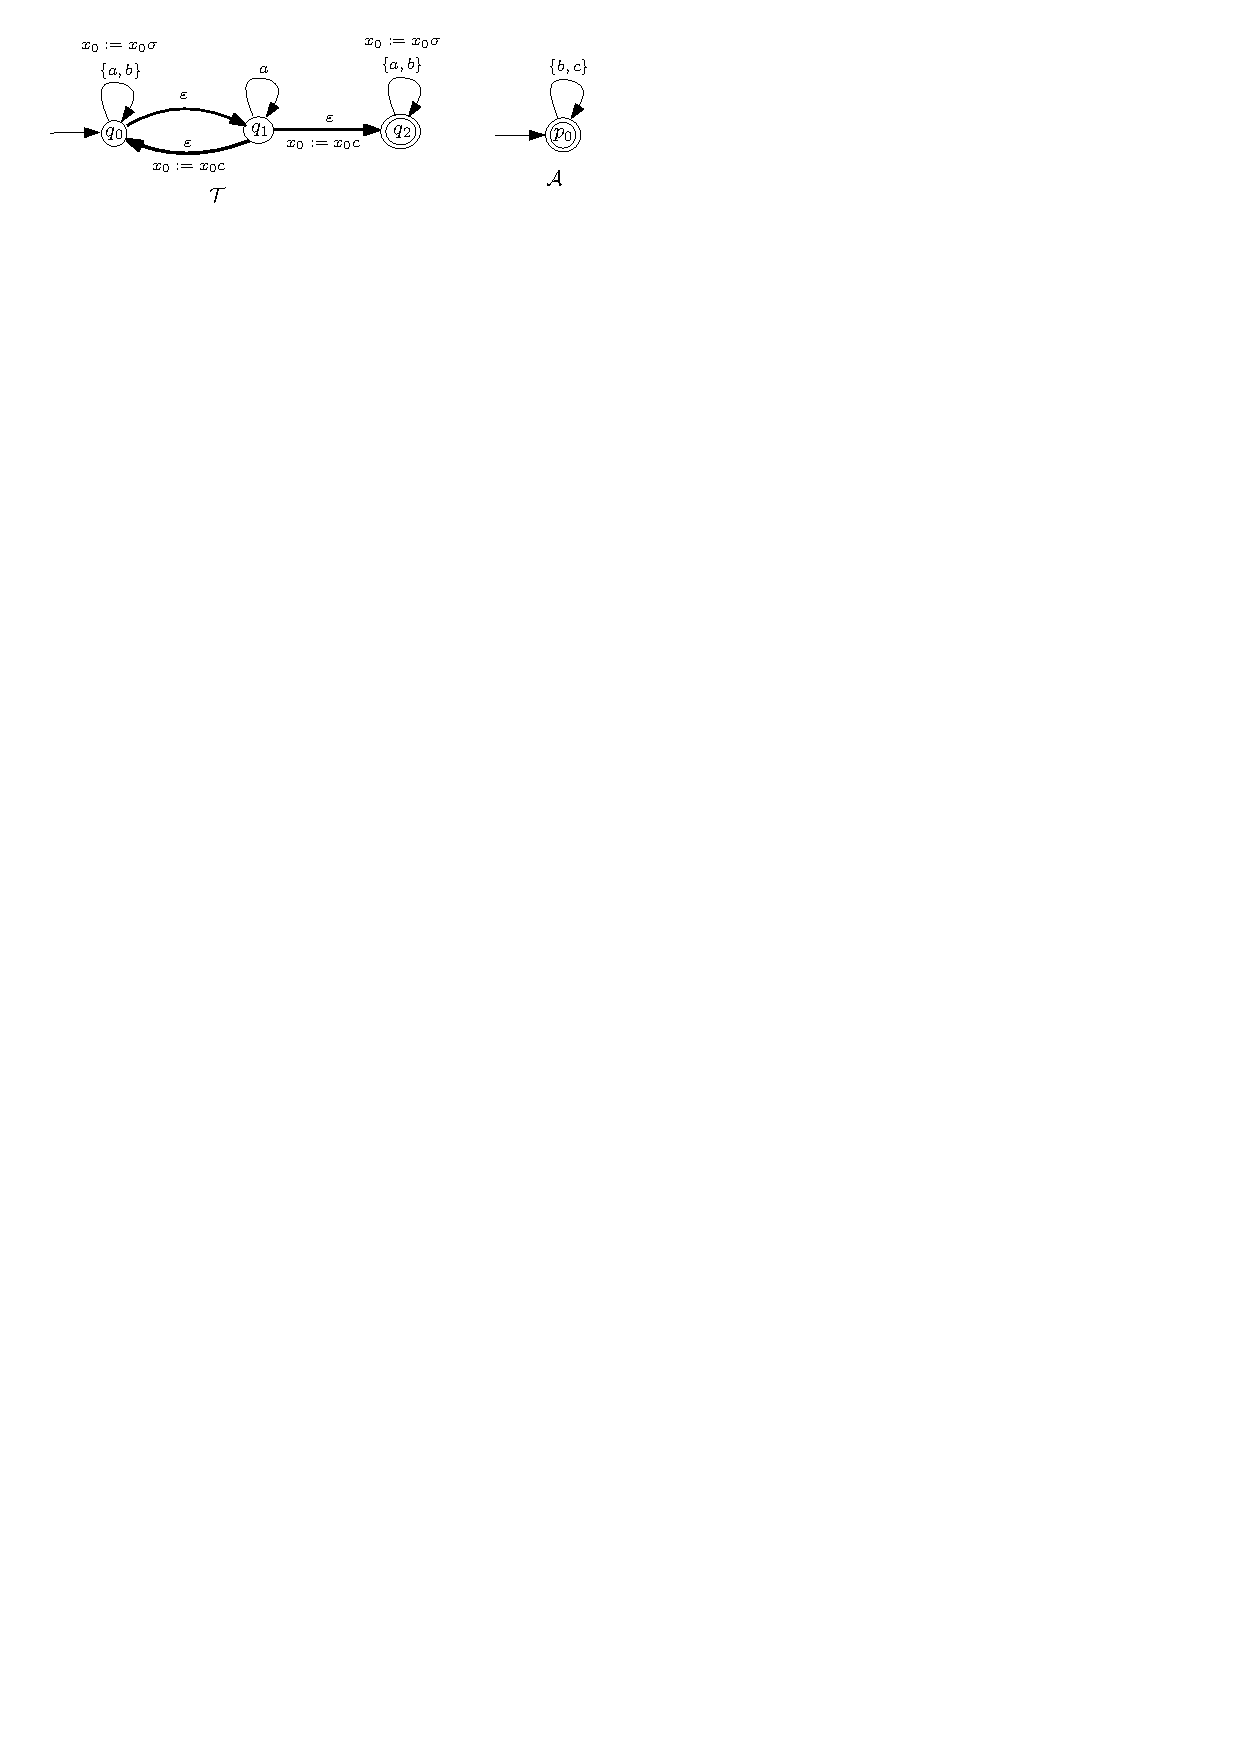
\includegraphics[scale=0.8]{pre-image-counter-example.pdf}
                \caption{A counterexample to disprove the flawed pre-image construction method}
                \label{fig-pre-image-count-exmp}
            \end{figure}
            }
            %%%%%%%%%%%%%%%%%%%%%%%%%%%%%%%%
            %%%%%%%%%%%%%%%%%%%%%%%%%%%%%%%%

            %\begin{proof}[Lemma~\ref{lem:psst_preimage}]

            %We are ready to prove Lemma~\ref{lem:psst_preimage}.

            %Let $\psst = (Q_T, \Sigma$, $X, \delta_T, \tau_T, E_T,  q_{0, T}, F_T)$ be a PSST and $\Aut= (Q_A, \Sigma, \delta_A, q_{0, A}, F_A)$ be an \FA{}.
            While the aforementioned natural idea does not work,  we choose to construct an FA $\cB$ that simulates the \emph{accepting} run of $\psst$ on $w$, and, for each $x \in X$, records an $\Aut$-abstraction of the string stored in $x$, that is, the set of state pairs $(p, q) \in Q_A \times Q_A$ such that starting from $p$, $\Aut$ can reach $q$ after reading the string stored in $x$.
            To simulate the accepting run of $\psst$, it is necessary to record all the states accessible through the runs of higher priorities to ensure the current run is indeed the accepting run of $\psst$ (of highest priority). Moreover, $\cB$ also remembers the set of $\varepsilon$-transitions of $\cT$ after the latest non-$\varepsilon$-transition to ensure that no transition occurs twice in a sequence of $\varepsilon$-transitions of $\cT$.

            Specifically, each state of $\cB$ is of the form $(q, \rho, \Lambda, S)$, where $q \in Q_T$, $\rho \in (\cP(Q_A \times Q_A ))^{X}$, $\Lambda \subseteq \cE(\tau_T)$, and $S \subseteq Q_T$.
            For a state $(q, \rho, \Lambda, S)$, our intention for $S$ is that the states in it are those that can be reached in the runs of higher priorities than the current run, by reading the same sequence of letters and applying the $\varepsilon$-transitions as many as possible. Note that when recording in $S$ all the states accessible through the runs of higher priorities, we do not take the non-repetition of $\varepsilon$-transitions into consideration since if a state is reachable by a sequence of $\varepsilon$-transitions where some $\varepsilon$-transitions are repeated, then there exists also a sequence of non-repeated $\varepsilon$-transitions reaching the state.
            Moreover, when simulating an $a$-transition of $\cT$ (where $a \in \Sigma$) at a state $(q, \rho, \Lambda, S)$, suppose $\delta_T(q, a) = (q_1, \cdots, q_m)$ and $\tau_T(q) = (P_1, P_2)$, then $\cB$ nondeterministically chooses $q_i$ and goes to the state $(q_i, \rho', \emptyset, S')$, where
            \begin{itemize}
                \item $\rho'$ is obtained from $\rho$ and $E_T(q, \sigma, q_i)$,
                    %
                \item $\Lambda$ is reset to $\emptyset$,
                    %
                \item all the states obtained from $S$ by applying  an $a$ transition should be \emph{saturated by $\varepsilon$-transitions} and put into $S'$, more precisely, all the states reachable from $S$ by first applying an $a$-transition, then a sequence of $\varepsilon$-transitions, should be put into $S'$,
                    %
                \item moreover, all the states obtained from $q_1,\cdots, q_{i-1}$ (which are of higher priorities than $q_i$) by saturating with $\varepsilon$-transitions should be put into $S'$,
                    %
                \item finally, all the states obtained from those in $P'_1 = \{q' \in P_1 \mid (q, q') \not \in \Lambda\}$ (which are of higher priorities than $q_i$) by saturating with non-$\Lambda$ $\varepsilon$-transitions first (i.e. the $\varepsilon$-transitions that do not belong to $\Lambda$), and applying an $a$-transition next, finally saturating with $\varepsilon$-transitions again, should be put into $S'$, (note that according to the semantics of PSST, the $\varepsilon$-transitions in $\Lambda$ should be avoided when defining $P'_1$ and saturating the states in $P'_1$ with $\varepsilon$-transitions).
            \end{itemize}
            %For technical reasons, when constructing $\cB$, we assume that this saturation happens when a state is added to $S$ for the first time. Therefore, at a state $(q, \rho, \Lambda, S)$, all the states reachable from the states in $S$ by sequences of $\varepsilon$-transitions in $\cT$ have already been in $S$.

            The above construction  does not utilize the so-called \tmtextit{copyless} property (i.e. for each transition $t$ and each variable $x$, $x$ appears at most once on the right-hand side of the assignment for $t$) \cite{AC10,AD11},
            thus it works for general, or \textit{copyful}, PSSTs \cite{FR17}.
            It can be noted that the powerset in
            $\rho \in (\cP(Q_A \times Q_A ))^{X}$
            is required to handle copyful transductions as the contents of a variable may be used in many different situations, each requiring a different abstraction.
            If the PSST is copyless, we can instead use
            $\rho \in (Q_A \times Q_A)^{X}$.
            That is, each variable is used only once, and hence only one abstraction pair is needed.
            The powerset construction in the transitions can be replaced by a non-deterministic choice of the particular pair of states from $Q_A$ that should be kept.
            This avoids the construction being exponential in the size of $A$, which in turn avoids the tower of exponential blow-up in the backwards reasoning.

            %The formal construction of $\cB$ is omitted, due to the page limit. The interested readers can read Appendix~\ref{app-pre-image} for more details.

            %%%%%%%%%%%%%%%%%%%%%%%%%%%%%%%%%%%
            %%%%%%%%%%%%%%%%%%%%%%%%%%%%%%%%%%%
            \hide{
                \begin{table}[t]
                    \centering
                    \caption{the actual $\cB$ state in Figure
                    \label{table:psst-preimage}
                    \ref{fig-psst-preimage-exmp}}
                    \begin{tabular}{|c|c|}
                        \hline
                        Symbol & State of $\cB$\\
                        \hline
                        $r_0$ & $(q_0, \rho_1, \emptyset, \emptyset)$\\
                        \hline
                        $r_1$ & $(q_1, \rho_1, \{ (q_0, q_1) \}, \emptyset)$\\
                        \hline
                        $r_2$ & $(q_2, \rho_1, \{ (q_0, q_1), (q_1, q_2) \}, \{ q_0 \})$\\
                        \hline
                        $r_3$ & $(q_2, \rho_2, \emptyset, \{ q_0, q_1, q_2 \})$\\
                        \hline
                        $r_4$ & $(q_2, \rho_1, \emptyset, \{ q_0, q_1, q_2 \})$\\
                        \hline
                        $r_5$ & $(q_0, \rho_1, \{ (q_0, q_1) (q_1, q_0) \}, \emptyset)$\\
                        \hline
                        $r_6$ & $(q_0, \rho_2, \emptyset, \emptyset)$\\
                        \hline
                        $r_7$ & $(q_0, \rho_2, \emptyset, \{ q_0, q_1, q_2 \})$\\
                        \hline
                        $r_8$ & $(q_1, \rho_2, \{ (q_0, q_1) \}, \{ q_0, q_1, q_2 \})$\\
                        \hline
                        $r_9$ & $(q_0, \rho_2, \{ (q_0, q_1) (q_1, q_0) \}, \{ q_0, q_1, q_2 \})$\\
                        \hline
                        $r_{10}$ & $(q_2, \rho_2, \{ (q_0, q_1) (q_1, q_2) \}, \{ q_0, q_1, q_2 \})$\\
                        \hline
                        $r_{11}$ & $(q_0, \rho_1, \emptyset, \{ q_0, q_1, q_2 \})$\\
                        \hline
                        $r_{12}$ & $(q_1, \rho_1, \{ (q_0, q_1) \}, \{ q_0, q_1, q_2 \})$\\
                        \hline
                        $r_{13}$ & $(q_0, \rho_1, \{ (q_0, q_1) (q_1, q_0) \}, \{ q_0, q_1, q_2 \})$\\
                        \hline
                        $r_{14}$ & $(q_2, \rho_1, \{ (q_0, q_1) (q_1, q_2) \}, \{ q_0, q_1, q_2 \})$\\
                        \hline
                        $r_{15}$ & $(q_2, \rho_2, \{ (q_0, q_1) (q_1, q_2) \}, \{ q_0 \})$\\
                        \hline
                        $r_{16}$ & $(q_1, \rho_2, \emptyset, \{ q_0, q_1, q_2 \})$\\
                        \hline
                        $r_{17}$ & $(q_2, \rho_2, \{ (q_1, q_2) \}, \{ q_0, q_1, q_2 \})$\\
                        \hline
                        $r_{18}$ & $(q_0, \rho_2, \{ (q_1, q_0) \}, \{ q_0, q_1, q_2 \})$\\
                        \hline
                        $r_{19}$ & $(q_1, \rho_2, \{ (q_1, q_0) (q_0, q_1) \}, \{ q_0, q_1, q_2 \})$\\
                        \hline
                        $r_{20}$ & $(q_2, \rho_2, \{ (q_1, q_0) (q_0, q_1) (q_1, q_2) \}, \{ q_0, q_1, q_2 \})$\\
                        \hline
                        $r_{21}$ & $(q_1, \rho_2, \{ (q_0, q_1) \}, \emptyset)$\\
                        \hline
                        $r_{22}$ & $(q_0, \rho_2, \{ (q_0, q_1) (q_1, q_0) \}, \emptyset)$\\
                        \hline
                    \end{tabular}
                \end{table}
                }
                %%%%%%%%%%%%%%%%%%%%%%%%%%%%%%%%%%%
                %%%%%%%%%%%%%%%%%%%%%%%%%%%%%%%%%%%

                %
                %\zhilin{stopped here}
                %\zhilei{changed a little bit}

                %%%%%%%%%%%%%%%%%%%%%%%%%%%%%%%%%%%%%%%%%
                %%%%%%%%%%%%%%%%%%%%%%%%%%%%%%%%%%%%%%%%%
                \hide{
                    \subsection{Complexity}

                    \begin{proposition}[POPL'19]
                        The path feasibility problem of the following two fragments is non-elementary: SL with 2FTs, and SL with FTs+replaceAll.

                        SL[conc, replaceAll, reverse, FFT] is expspace-complete (note that 2FTs in SL are restricted to be one-way and functional)
                    \end{proposition}

                    %The same proof strategy can be used for FTs+replaceAll. The 2FTs used in the proof above
                    %proceed by running completely over the word and producing some output, then silently moving
                    %back to the beginning of the word. An arbitrary number of passes are made in this way. We
                    %can simulate this behaviour using FTs and replaceAll.


                    The main open question is the complexity of the SL fragment with replaceall function and prioritized streaming transducers. Note that PSST can simulate 2FT (adapting Matt's proof?), so we could obtain nonelementary lower bound for SL with PSST.

                    However, this variant of replaceall is quite different from the replaceall we had before ...

                    \begin{enumerate}
                        \item  does  copyless help?
                        \item how about SL with only this version of replaceall?
                    \end{enumerate}
                    }
                    %%%%%%%%%%%%%%%%%%%%%%%%%%%%%%%%%%%%%%%%%
                    %%%%%%%%%%%%%%%%%%%%%%%%%%%%%%%%%%%%%%%%%


                    %Let $\psst = (Q_T, \Sigma$, $X, \delta_T, \tau_T, E_T,  q_{0, T}, F_T)$ be a PSST  and $\Aut
                    %  = (Q_A, \Sigma$, $\delta_A$, $q_{0, A}$, $F_A)$ be an \FA{}. Without loss of generality, we assume that $\Aut$ contains no $\varepsilon$-transitions. For convenience, we use $\cE(\tau_T)$ to denote $\{(q, q') \mid q' \in \tau_T(q)\}$.

                    For the formal construction of $\cB$, we need some additional notations.
                    \begin{itemize}
                        \item For $S \subseteq Q_T$, $\delta^{(ip)}_T(S, a) = \{q'_1 \mid \exists q_1 \in S, q'_1 \in \delta_T(q_1, a)\}$.
                            %
                        \item For $q \in Q_T$,  if $\tau_T(q) = (P_1, P_2)$, then $\tau^{(ip)}_T(\{q\})=S$ such that $S = P_1 \cup P_2$.
                            Moreover, for $S \subseteq Q_T$, we define $\tau^{(ip)}_T(S) = \bigcup \limits_{q \in S} \tau^{(ip)}_T(\{q\})$. We also use $\big(\tau^{(ip)}_T\big)^\ast$ to denote the $\varepsilon$-closure of $\cT$, namely, $\big(\tau^{(ip)}_T\big)^\ast(S) = \bigcup \limits_{n \in \Nat} \big(\tau^{(ip)}_T\big)^{n}(S)$, where $\big(\tau^{(ip)}_T\big)^{0}(S) = S$, and for $n \in \Nat$, $\big(\tau^{(ip)}_T\big)^{n+1}(S) = \tau^{(ip)}_T\big(\big(\tau^{(ip)}_T\big)^{n}(S)\big)$.
                            %
                        \item For $S \subseteq Q_T$ and $\Lambda \subseteq  \cE(\tau_T)$, we use $\big(\tau^{(ip)}_T \backslash \Lambda\big)^\ast(S)$ to denote the set of states reachable from $S$ by sequences of $\varepsilon$-transitions where {\it no} transitions $(q, \varepsilon, q')$ such that $(q, q') \in \Lambda$ are used.
                            %
                            %We also use $(\tau^{(ip)}_T)^\ast$ to denote the reflexive transitive closure of $\tau^{(ip)}_T$. \tl{here $(\tau^{(ip)}_T)$ is defined as a function... you mean function composition?}
                            %\zhilei{I think we can just use the term 'epsilon closure' here?}
                            %\item For $\sigma \in \Sigma$ and $S \subseteq Q_T$,  we use $\tau^+_T[a, S]$ to denote the set of states that can be obtained from
                            %
                        \item For $\rho \in (\cP(Q_A \times Q_A ))^{X}$ and $s \in X \rightarrow (X \cup \Sigma)^{\ast}$, we use $s(\rho)$ to denote $\rho'$ that is obtained from $\rho$ as follows: For each $x \in X$, if $s(x) = \varepsilon$, then $\rho'(x) = \{(p, p) \mid p \in Q_A\}$, otherwise, let $s(x) = b_1 \cdots b_\ell$ with $b_i \in \Sigma \cup X$ for each $i \in [\ell]$, then $\rho'(x) = \theta_1 \circ \cdots \circ \theta_\ell$, where $\theta_i = \delta^{(b_i)}_A$ if $b_i \in \Sigma$, and $\theta_i = \rho(b_i)$ otherwise, and $\circ$ represents the composition of binary relations.
                    \end{itemize}

                    We are ready to present the formal construction of $\cB =  (Q_B$, $\Sigma$, $\delta_B$, $q_{0, B}, F_B)$.
                    \begin{itemize}
                        \item $Q_B = Q_T \times (\cP(Q_A \times Q_A ))^{X} \times \cP(\cE(\tau_T)) \times \cP(Q_T)$,
                            %(Intuitively, the letter $\sigma$ in $(q, \sigma, \rho, S) \in Q_B$ means the next letter to be read at $q$, with $\bot$ represents the end of the input.)

                        \item $q_{0, B} = (q_{0,T}, \rho_{\varepsilon}, \emptyset, \emptyset)$ where $\rho_{\varepsilon} (x) = \{(q, q) \mid q \in Q\}$ for each $x \in X$,

                        \item $\delta_{B}$ comprises
                            \begin{itemize}
                                    %\item the tuples $(q'_0, \varepsilon, ((q_{0,T},\sigma), \rho_{\varepsilon}, \emptyset))$ where $\sigma \in \Sigma$, $\rho_{\varepsilon} (x) = \{(q, q) \mid q \in Q\}$ for each $x \in X$,
                                    %
                                \item the tuples $((q, \rho, \Lambda, S), a, (q_i, \rho', \Lambda', S'))$ such that
                                    %there exists $s \in \left((X \cup \Sigma\right)^*)^X)$ satisfying
                                    \begin{itemize}
                                        \item $a \in \Sigma$,
                                            %$a' \in \Sigma \cup \{\bot\}$,
                                            %
                                        \item $\delta_T (q, a) = (q_1, \ldots, q_i, \ldots, q_m)$,
                                            %
                                        \item $s = E((q, a, q_i))$,
                                            %
                                        \item $\rho' = s(\rho)$,
                                            %
                                        \item $\Lambda' = \emptyset$, (Intuitively, $\Lambda$ is reset.)
                                            %
                                        \item let $\tau_T(q) = (P_1, P_2)$, then $S' = \big(\tau^{(ip)}_T\big)^\ast\big(\{ q_1$, $\ldots$, $q_{i - 1} \} \cup \delta^{(ip)}_T\big(S \cup \big(\tau^{(ip)}_T \setminus \Lambda\big)^\ast(P'_1), a\big)\big)$, where $P'_1 = \{q' \in P_1 \mid (q, q') \not \in \Lambda\}$;
                                            %(Note that according to the semantics of PSSTs, when computing the set of states reachable from $q$ through an $\varepsilon$-transition to some $q' \in P_1$ first and a sequence of $\varepsilon$-transitions starting from $q'$ next, the transitions $(q'', \varepsilon, q''')$ with $(q'', q''') \in \Lambda$ should be excluded. )
                                            %
                                    \end{itemize}
                                    %
                                \item the tuples $((q, \rho, \Lambda, S), \varepsilon, (q_i, \rho', \Lambda', S'))$ such that
                                    %there exists $s \in \left((X \cup \Sigma\right)^*)^X$ satisfying
                                    \begin{itemize}
                                            %, $a' \in \Sigma \cup \{\bot\}$,
                                            %
                                        \item $\tau_T(q) = ((q_1, \ldots, q_i, \ldots, q_m); \cdots)$,
                                            %
                                        \item $(q, q_i) \not \in \Lambda$,

                                        \item $s = E(q, \varepsilon, q_i)$,
                                            %
                                        \item $\rho' = s(\rho)$,
                                            %
                                        \item $\Lambda' = \Lambda \cup \{(q, q_i)\}$,
                                            %
                                        \item $S' =  S \cup \big(\tau^{(ip)}_T \backslash \Lambda \big)^\ast(\{ q_j \mid j \in [i-1], (q, q_j) \not \in \Lambda \})$;
                                            %
                                            %$\rho'(x) = \theta_\ell$ such that $\theta_0 = \{(p,p) \mid p \in Q_A\}$, and for each $i \in [\ell]$, if $b_i \in \Sigma$, then $\theta_i = \{(p, p') \mid (p, p'') \in \theta_{i-1}, (p'', b_i, p') \in \delta_A \mbox{ for some } p''\}$, otherwise, $\theta_i = \theta_{i-1} \cdot \rho(x)$.
                                    \end{itemize}
                                    %

                                \item the tuples $((q, \rho, \Lambda, S), \varepsilon, (q_i, \rho', \Lambda', S'))$ such that
                                    %there exists $s \in \left((X \cup \Sigma\right)^*)^X$ satisfying
                                    \begin{itemize}
                                            %\item $a \in \Sigma$,
                                            %$a' \in \Sigma \cup \{\bot\}$,
                                            %
                                        \item $\tau_T (q) = ((q'_1, \ldots, q'_n); (q_1, \ldots, q_i, \ldots, q_m))$,
                                            %
                                        \item $(q, q_i) \not \in \Lambda$,
                                            %
                                        \item $s = E(q, \varepsilon, q_i)$,
                                            %
                                        \item $\rho' = s(\rho)$,
                                            %
                                        \item $\Lambda' = \Lambda \cup \{(q, q_i)\}$,
                                            %
                                        \item $S' = S \cup \{q\} \cup \big(\tau^{(ip)}_T \backslash \Lambda \big)^\ast\big(\big\{q'_j \mid j \in [n], (q, q'_j) \not \in \Lambda \big\} \cup \big\{q_j \mid j \in [i-1], (q, q_j) \not \in \Lambda \big\} \big)$. (Note that here we include $q$ into $S'$, since the non-$\varepsilon$-transitions out of $q$ have higher priorities than the transition $(q, \varepsilon, q_i)$.)
                                            %
                                            %$\rho'(x) = \theta_\ell$ such that $\theta_0 = \{(p,p) \mid p \in Q_A\}$, and for each $i \in [\ell]$, if $b_i \in \Sigma$, then $\theta_i = \{(p, p') \mid (p, p'') \in \theta_{i-1}, (p'', b_i, p') \in \delta_A \mbox{ for some } p''\}$, otherwise, $\theta_i = \theta_{i-1} \cdot \rho(x)$.
                                    \end{itemize}
                            \end{itemize}
                        \item
                            Moreover, $F_B$ is the set of states $(q, \rho, \Lambda, S) \in Q_B$ such that
                            \begin{enumerate}
                                \item $F_T (q)$ is defined,
                                    %
                                \item for every $q' \in S$, $F_T (q')$ is not defined,
                                    %
                                \item if $F_T(q) = \varepsilon$, then $q_{0, A}  \in F_A$, otherwise,
                                    let $F_T(q) = b_1 \cdots b_\ell$ with $b_i \in \Sigma \cup X$ for each $i \in [\ell]$, then $(\theta_1 \circ \cdots \circ \theta_\ell) \cap (\{q_{0,A}\} \times F_A) \neq \emptyset$, where for each $i \in [\ell]$, if $b_i \in \Sigma$, then $\theta_i = \delta^{(b_i)}_A$, otherwise, $\theta_i = \rho(b_i)$.
                            \end{enumerate}
                    \end{itemize}
                    %\end{proof}

\OMIT{
                    \begin{example}
                        Let us continue Example~\ref{pre-image-count-examp}. Suppose $\cT_{\tt extract_{decimalReg,1}} = (Q_T, \Sigma$, $X, \delta_T$, $\tau_T, E_T,  q_{0, T}, F_T)$. Then the FA defining $\cR^{-1}_{\cT_{\tt extract_{decimalReg,1}}}(\Lang(\Aut))$ constructed by using the aforementioned procedure is illustrated in Fig. \ref{fig-psst-preimage-exmp}, where the final states are those doubly boxed states, moreover, the states reachable from the state $(q_2, \emptyset, \{(q_1,q_2)\}, \{q_1\})$ are omitted because no final states are unreachable from those states, which are therefore redundant. Let us exemplify the construction by considering the state $(q_5, \{(p_0,p_0)\}, \{(q_1,q_2), (q_2,q_3), (q_3,q_4), (q_4, q_5)\}, \{q_1,q_3\})$. For each letter $\ell \in \{0,\cdots, 9\}$, the state $(q_5, \{(p_0,p_0)\}, \emptyset, \{q_1,q_2, q_3, q_4, q_5, q_6\})$ is reached from it, since $\delta_T(q_5,\ell)  = (q_5)$, $\delta_T(q_1,\ell) = (q_1)$ and $(\tau^{(ip)}_T)^*(\{q_1\}) = \{q_1, q_2, q_3, q_4, q_5, q_6\}$. The state $(q_6, \{(p_0,p_0)\}, \{(q_5,q_6)\}, \{q_1, q_2, q_3, q_4, q_5, q_6\})$ is not a final state since $q_6$ is in $\{q_1, q_2, q_3, q_4, q_5, q_6\}$ and $F_T(q_6)$ is defined.
                        %For efficiency, we minimize the FA after the construction. See Section \ref{sect:impl} for implementation details.
                        %
                        \begin{figure}[ht]
                            \centering
                            %\rule{\linewidth}{0cm}

                            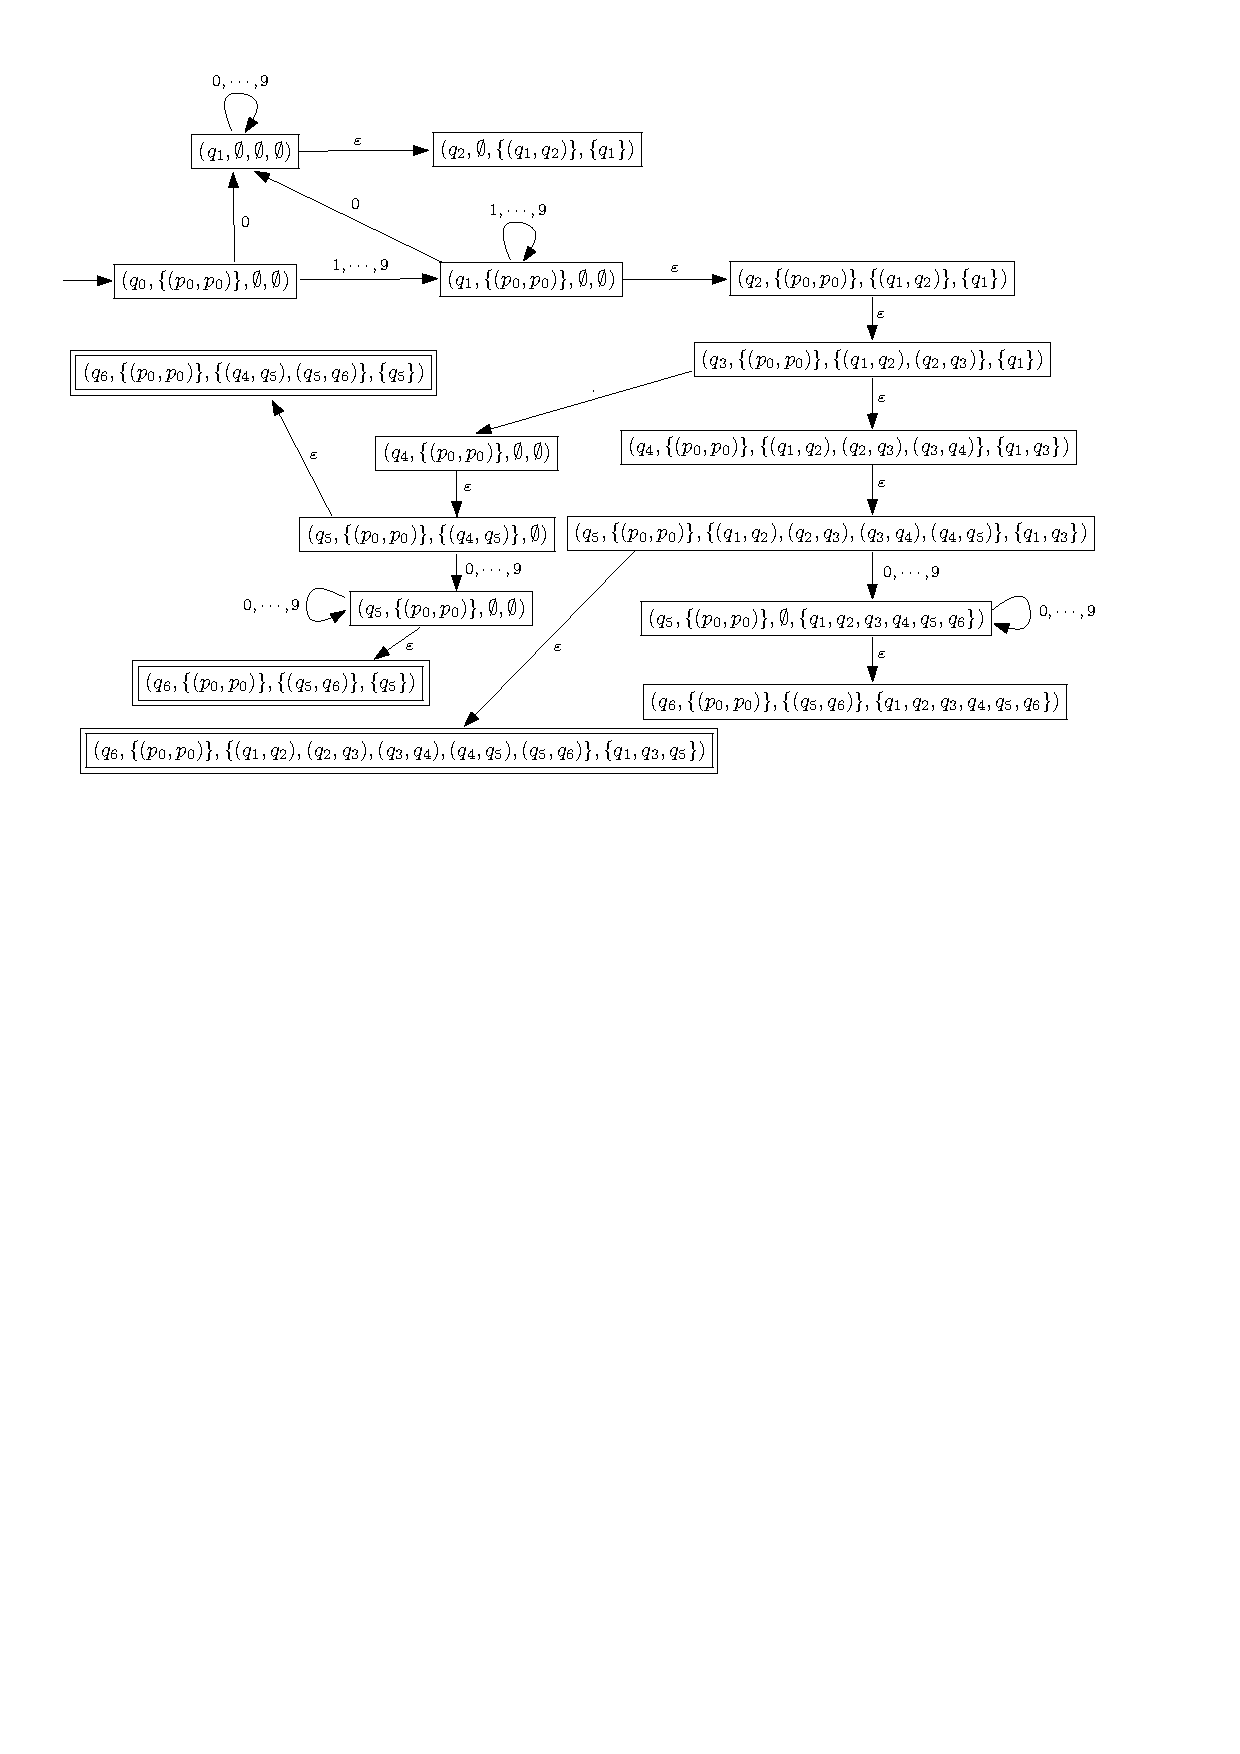
\includegraphics[width = \textwidth]{psst-preimage-example-new.pdf}
                            \caption{The FA defining $\cR^{-1}_{\cT_{\tt extract_{decimalReg,1}}}(\Lang(\Aut))$}
                            \label{fig-psst-preimage-exmp}
                        \end{figure}
                    \end{example}

                    \begin{remark}
                        The computation of the pre-image of an FA $\cA$ under a PSST $\cT$ can be understood from a different angle: At first, $\cT$ can be turned into an equivalent a streaming string transducer $\cT'$, then the pre-image of $\cA$ under $\cT'$ is computed. Therefore, from the viewpoint of expressibility, PSSTs and SSTs are equivalent. Nevertheless, PSSTs are exponentially more succinct than SSTs, moreover, the priorities in PSSTs are very convenient for modeling the greedy/lazy semantics of Kleene star.
                    \end{remark}
}

                    %%%%%%%%%%%%%%%%%%%%%%%%%%%%%%%%%%%%%%%%%%%%%
                    %%%%%%%%%%%%%%%%%%%%%%%%%%%%%%%%%%%%%%%%%%%%%
                    \hide{
                        \subsection{Experiment result of Aratha and Expose}

                        \begin{table}[H]
                            \begin{center}
                                \begin{tabular}{l@{\quad}c@{\quad}|*{2}{c}|@{\quad}*{2}{c}}
                                    & &
                                    \multicolumn{2}{c|@{\quad}}{\textbf{ExpoSE}} &\multicolumn{2}{c@{\quad}}{\textbf{Aratha}}
                                    \\
                                    & \#Benchm. &  ~~\# Excuted ~~ & ~~\#Timeout~~ &  ~~\# Excuted ~~ & ~~\#Timeout
                                    \\\hline
                                    \textbf{Regex-ExpoSE} & 94 & 93 & 1 & \textbf{94} & 0
                                    \\
                                    && \multicolumn{2}{c|@{\quad}}{Average time: 17.65s} & \multicolumn{2}{c@{\quad}}{Average time: \textbf{5.53} s}
                                    \\\hline
                                    \textbf{Replace-JS} & 40 & 16 & 24 & \textbf{40} & 0
                                    \\
                                    && \multicolumn{2}{c|@{\quad}}{Average time: 17.65s} & \multicolumn{2}{c@{\quad}}{Average time: \textbf{2.69}s}
                                    \\\hline
                                    \textbf{Match-JS} & 38 &  30&   8& \textbf{38} & 0
                                    \\
                                    && \multicolumn{2}{c|@{\quad}}{Average time: 13.56s} & \multicolumn{2}{c@{\quad}}{Average time: \textbf{2.78}s}
                                    \\
                                \end{tabular}
                            \end{center}
                            \caption{Results of running javascript program on Aratha and Expose. The core smt solver of Aratha is \ostrich. Average time does not count timeout files and the time limit is 60s. All epxeriments were done on an Intel-Xeon-E5-2690-@2.90GHz machine, running 64-bit Linux and Java 1.8.}
                            \label{tab:exp}
                        \end{table}
                        }
                        %%%%%%%%%%%%%%%%%%%%%%%%%%%%%%%%%%%%%%%%%%%%%
                        %%%%%%%%%%%%%%%%%%%%%%%%%%%%%%%%%%%%%%%%%%%%%
